\section{บทที่ 1 บทนำคณิตศาสตร์สำหรับวิศวกรรมไฟฟ้าและเครื่องมือคำนวณ}

\textbf{ชื่อบทภาษาอังกฤษ:} Introduction to Electrical Engineering Mathematics and Computational Tools
\textbf{รายวิชา:} คณิตศาสตร์วิศวกรรมไฟฟ้า (Electrical Engineering Mathematics)
\textbf{รหัสวิชา:} 5571102
\textbf{สาขาวิชา:} เทคโนโลยีวิศวกรรมไฟฟ้า
\textbf{คณะ:} เทคโนโลยีอุตสาหกรรม
\textbf{ภาคเรียนที่:} 1
\textbf{ปีการศึกษา:} 2569
\textbf{ระดับผู้เรียน:} นักศึกษาระดับปริญญาตรี สาขาวิชาเทคโนโลยีวิศวกรรมไฟฟ้า
\textbf{จำนวนชั่วโมงที่แนะนำ:} 3 ชั่วโมงสำหรับสัปดาห์ที่ 1 (เป็นข้อเสนอเชิงออกแบบการสอนจากแผนรายสัปดาห์)
\textbf{ความยาวเป้าหมาย:} 25–30 หน้า A4 โดยประมาณเมื่อจัดหน้าด้วยฟอนต์ TH Sarabun New หรือเทียบเท่า ขนาดเนื้อหา 16 pt
\textbf{รูปแบบการเรียน:} บรรยายร่วมกับการคำนวณ การอภิปราย และการสาธิตเครื่องมือคำนวณ
\textbf{โหมดการออกแบบ:} Hybrid Mode

\par\noindent\rule{\textwidth}{0.4pt}\par

\subsection{1. แนวคิดสำคัญของบท}

คณิตศาสตร์เป็นภาษากลางของวิศวกรรมไฟฟ้า เพราะปริมาณทางไฟฟ้า เช่น แรงดัน กระแส กำลัง พลังงาน ความถี่ มุมเฟส และสนามแม่เหล็กไฟฟ้า ล้วนต้องอาศัยสัญลักษณ์ สมการ ฟังก์ชัน กราฟ และแบบจำลองเพื่ออธิบายความสัมพันธ์อย่างเป็นระบบ การเรียนคณิตศาสตร์สำหรับวิศวกรรมไฟฟ้าจึงไม่ควรจำกัดอยู่ที่การแทนค่าในสูตร แต่ต้องพัฒนาไปสู่ความสามารถในการ \textbf{อ่านปัญหา สร้างแบบจำลอง เลือกวิธีคำนวณ ตรวจสอบหน่วย ประเมินความสมเหตุสมผล และแปลความหมายผลลัพธ์กลับสู่ระบบจริง}

บทนี้ทำหน้าที่เป็นสะพานเชื่อมระหว่างคณิตศาสตร์พื้นฐานที่ผู้เรียนเคยเรียนกับหัวข้อเฉพาะทางในรายวิชา ได้แก่ จำนวนเชิงซ้อนและเฟสเซอร์ การวิเคราะห์เวกเตอร์ อนุกรมฟูเรียร์ การแปลงลาปลาซ และการใช้โปรแกรมคำนวณทางวิศวกรรม โดยเน้นการทบทวนพีชคณิต ฟังก์ชัน กราฟ หน่วยทางวิศวกรรม การประมาณค่า และการใช้สัญญาณไซน์เป็นตัวอย่างสำคัญในการเชื่อมโยงคณิตศาสตร์กับระบบไฟฟ้ากระแสสลับ

ผู้เรียนจะได้เห็นว่าเครื่องมือคำนวณ เช่น เครื่องคิดเลขวิทยาศาสตร์ Python, MATLAB, GNU Octave และเครื่องมือแบบ Notebook มีบทบาทในการช่วยคำนวณและสร้างภาพ แต่ไม่สามารถทดแทนการวิเคราะห์ทางวิศวกรรมได้อย่างสมบูรณ์ ผลจากซอฟต์แวร์จะมีความหมายก็ต่อเมื่อผู้ใช้กำหนดสมการ หน่วย เงื่อนไข และตีความผลลัพธ์ได้ถูกต้อง

\textbf{แก่นของบทนี้มี 4 ประเด็น}

\begin{enumerate}
    \item คณิตศาสตร์เป็นเครื่องมือสำหรับอธิบาย วิเคราะห์ และออกแบบระบบไฟฟ้า
    \item หน่วย สัญลักษณ์ ฟังก์ชัน และกราฟเป็นองค์ประกอบพื้นฐานของการสื่อสารทางวิศวกรรม
    \item การคำนวณที่ดีต้องมีทั้งความถูกต้องเชิงตัวเลขและความสมเหตุสมผลเชิงกายภาพ
    \item โปรแกรมคำนวณเป็นเครื่องมือสนับสนุนกระบวนการคิด ไม่ใช่สิ่งทดแทนความเข้าใจหลักการ
\end{enumerate}

\par\noindent\rule{\textwidth}{0.4pt}\par

\subsection{2. ความรู้พื้นฐานก่อนเรียน}

ก่อนศึกษาบทนี้ ผู้เรียนควรมีพื้นฐานดังต่อไปนี้

\begin{itemize}
    \item การบวก ลบ คูณ หาร จำนวนจริง และเศษส่วน
    \item การแก้สมการเชิงเส้นอย่างง่าย
    \item เลขยกกำลัง รากที่สอง และสัญกรณ์วิทยาศาสตร์
    \item ฟังก์ชันพื้นฐานและการอ่านกราฟแกนพิกัดฉาก
    \item ตรีโกณมิติพื้นฐาน โดยเฉพาะฟังก์ชันไซน์และโคไซน์
    \item การแปลงหน่วยพื้นฐาน เช่น วินาที มิลลิวินาที โวลต์ มิลลิโวลต์ แอมแปร์ และมิลลิแอมแปร์
    \item การใช้เครื่องคิดเลขวิทยาศาสตร์ในโหมดองศาและเรเดียน
    \item ทักษะพื้นฐานในการใช้งานคอมพิวเตอร์หรือเว็บเบราว์เซอร์
\end{itemize}

ผู้เรียนที่ยังไม่มั่นใจเรื่องการจัดรูปสมการ การแปลงหน่วย หรือมุมองศา–เรเดียน ควรทบทวนส่วนดังกล่าวควบคู่กับหัวข้อ 7.4–7.6 ของบทนี้ เพราะเป็นทักษะที่ใช้ต่อเนื่องตลอดรายวิชา

\par\noindent\rule{\textwidth}{0.4pt}\par

\subsection{3. คำสำคัญประจำบท}

\begin{table}[htbp]
    \centering
    \begin{tabular}{l l l}
        \hline
        \textbf{คำภาษาไทย} & \textbf{คำภาษาอังกฤษ} & \textbf{ความหมายโดยย่อ} \\
        \hline
        คณิตศาสตร์วิศวกรรมไฟฟ้า & Electrical Engineering Mathematics & คณิตศาสตร์ที่ใช้สร้างแบบจำลอง วิเคราะห์ และแก้ปัญหาระบบไฟฟ้า \\
        ปริมาณทางไฟฟ้า & Electrical Quantity & ปริมาณที่ใช้บรรยายระบบไฟฟ้า เช่น แรงดัน กระแส กำลัง และพลังงาน \\
        หน่วยเอสไอ & SI Unit & หน่วยในระบบหน่วยสากลที่ใช้เป็นมาตรฐานในการวัดและสื่อสาร \\
        สัญญาณไฟฟ้า & Electrical Signal & ปริมาณไฟฟ้าที่เปลี่ยนแปลงตามตัวแปรอิสระ เช่น เวลา \\
        รูปคลื่น & Waveform & รูปร่างของสัญญาณเมื่อแสดงเป็นกราฟเทียบกับเวลา \\
        ฟังก์ชัน & Function & ความสัมพันธ์ที่กำหนดค่าผลลัพธ์จากค่าตัวแปรอิสระ \\
        สัญญาณไซน์ & Sinusoidal Signal & สัญญาณเป็นคาบที่อธิบายด้วยฟังก์ชันไซน์หรือโคไซน์ \\
        ค่าสูงสุด & Peak Value & ค่าสูงสุดของสัญญาณเมื่ออ้างอิงจากศูนย์ \\
        ค่ายอดถึงยอด & Peak-to-Peak Value & ผลต่างระหว่างยอดบวกสูงสุดกับยอดลบต่ำสุด \\
        ค่าประสิทธิผล & Root Mean Square: RMS & ค่าที่สัมพันธ์กับผลทางกำลังหรือความร้อนของสัญญาณในโหลดตัวต้านทาน \\
        ความถี่ & Frequency & จำนวนรอบของสัญญาณต่อวินาที หน่วยเฮิรตซ์ \\
        คาบเวลา & Period & เวลาที่สัญญาณใช้ครบหนึ่งรอบ \\
        ความถี่เชิงมุม & Angular Frequency & อัตราการเปลี่ยนแปลงของมุมเฟส หน่วยเรเดียนต่อวินาที \\
        มุมเฟส & Phase Angle & ตำแหน่งเชิงมุมของสัญญาณเมื่อเทียบกับจุดอ้างอิง \\
        การประมาณค่า & Approximation & การแทนค่าจริงด้วยค่าที่ใกล้เคียงภายใต้ความละเอียดที่เหมาะสม \\
        ความคลาดเคลื่อน & Error & ความแตกต่างระหว่างค่าประมาณ ค่าคำนวณ หรือค่าที่วัดกับค่าอ้างอิง \\
        การวิเคราะห์มิติ & Dimensional Analysis & การตรวจสอบความสอดคล้องของหน่วยหรือมิติในสมการ \\
        จำนวนเชิงซ้อน & Complex Number & จำนวนที่ประกอบด้วยส่วนจริงและส่วนจินตภาพ \\
        เฟสเซอร์ & Phasor & การแทนสัญญาณไซน์คงสถานะด้วยจำนวนเชิงซ้อนเพื่อสะดวกต่อการวิเคราะห์ \\
        เวกเตอร์ & Vector & ปริมาณที่มีทั้งขนาดและทิศทาง \\
        อนุกรมฟูเรียร์ & Fourier Series & การแทนฟังก์ชันเป็นคาบด้วยผลรวมขององค์ประกอบไซน์และโคไซน์ \\
        การแปลงลาปลาซ & Laplace Transform & เครื่องมือแปลงปัญหาจากโดเมนเวลาไปสู่โดเมนเชิงซ้อน $s$ \\
        โปรแกรมคำนวณ & Computational Tool & ซอฟต์แวร์หรือระบบที่ช่วยคำนวณ วิเคราะห์ สร้างกราฟ หรือจำลอง \\
        \hline
    \end{tabular}
\end{table}

\par\noindent\rule{\textwidth}{0.4pt}\par

\subsection{4. ผลลัพธ์การเรียนรู้ประจำบท}

\begin{quote}
เมื่อเรียนจบบทนี้ นักศึกษาสามารถ...
\end{quote}

\textbf{CLO1} อธิบายบทบาทของคณิตศาสตร์ต่อการสร้างแบบจำลองและการวิเคราะห์ปัญหาทางวิศวกรรมไฟฟ้าได้
\textbf{CLO2} เชื่อมโยงแนวคิดทางคณิตศาสตร์พื้นฐานกับงานวงจรไฟฟ้า สัญญาณไฟฟ้า สนามแม่เหล็กไฟฟ้า ระบบควบคุม และระบบไฟฟ้ากำลังได้
\textbf{CLO3} ใช้หน่วย สัญลักษณ์ สัญกรณ์วิทยาศาสตร์ และการแปลงหน่วยพื้นฐานทางวิศวกรรมไฟฟ้าได้อย่างถูกต้อง
\textbf{CLO4} ประยุกต์ใช้พีชคณิต ฟังก์ชัน กราฟ และสมการพื้นฐานเพื่อคำนวณและตีความปริมาณทางไฟฟ้าได้
\textbf{CLO5} เลือกใช้เครื่องคิดเลขหรือโปรแกรมคำนวณเบื้องต้นอย่างเหมาะสม พร้อมตรวจสอบผลลัพธ์ด้วยหน่วยและความสมเหตุสมผลทางกายภาพได้

\subsubsection{4.1 ตารางความสอดคล้องแบบ OBE}

\begin{table}[htbp]
    \centering
    \begin{tabular}{l l l l l}
        \hline
        \textbf{ผลลัพธ์การเรียนรู้ประจำบท} & \textbf{เนื้อหาที่เกี่ยวข้อง} & \textbf{กิจกรรมการเรียนรู้} & \textbf{วิธีประเมิน} & \textbf{หลักฐานการเรียนรู้} \\
        \hline
        CLO1 & 7.1, 7.2, 7.8 & อภิปรายบทบาทคณิตศาสตร์จากอุปกรณ์จริง & คำถามปากเปล่าและคำถามทบทวน & บันทึกการอภิปราย/คำตอบสั้น \\
        CLO2 & 7.2, 7.3, 7.10 & จับคู่เครื่องมือคณิตศาสตร์กับงานวิศวกรรม & ใบงานวิเคราะห์ความสัมพันธ์ & แผนผังหรือคำอธิบายความเชื่อมโยง \\
        CLO3 & 7.4, 7.6 & แบบฝึกแปลงหน่วยและตรวจหน่วย & แบบฝึกหัดพื้นฐาน & คำตอบพร้อมหน่วยและขั้นตอน \\
        CLO4 & 7.5, 7.9 & คำนวณสัญญาณไซน์และกำลังโหลด & แบบฝึกหัดคำนวณ/โจทย์วิเคราะห์ & วิธีทำ สมการ และการแปลผล \\
        CLO5 & 7.6, 7.7, 7.8 & ทดลองคำนวณและวาดกราฟด้วยซอฟต์แวร์ & งานสั้นหรือไฟล์ Notebook & กราฟ ผลคำนวณ และข้อความตรวจสอบความสมเหตุสมผล \\
        \hline
    \end{tabular}
\end{table}

\par\noindent\rule{\textwidth}{0.4pt}\par

\subsection{5. แผนผังเนื้อหาของบท}

ลำดับการเรียนรู้ของบทนี้ออกแบบจาก “ความหมาย” ไปสู่ “การคำนวณ” และต่อยอดสู่ “การใช้เครื่องมือ” ดังนี้

\textbf{บทบาทของคณิตศาสตร์}
→ \textbf{ความสัมพันธ์กับงานวิศวกรรมไฟฟ้า}
→ \textbf{ภาพรวมเครื่องมือคณิตศาสตร์ของรายวิชา}
→ \textbf{หน่วยและสัญลักษณ์พื้นฐาน}
→ \textbf{พีชคณิต ฟังก์ชัน กราฟ และสมการ}
→ \textbf{การคำนวณเชิงตัวเลขและการประมาณค่า}
→ \textbf{เครื่องมือคำนวณทางคณิตศาสตร์}
→ \textbf{กระบวนการแก้ปัญหาเชิงวิศวกรรม}
→ \textbf{ตัวอย่างวงจรและสัญญาณ}
→ \textbf{เชื่อมโยงสู่จำนวนเชิงซ้อน เวกเตอร์ ฟูเรียร์ และลาปลาซ}

% [รูปที่ 1: แผนผังความเชื่อมโยงคณิตศาสตร์กับงานวิศวกรรมไฟฟ้า]
% ประเภทภาพ: Infographic / Concept Map
% ตำแหน่งที่แนะนำ: หลังหัวข้อ 5 แผนผังเนื้อหาของบท
% วัตถุประสงค์การเรียนรู้: ช่วยให้ผู้เรียนเห็นว่าคณิตศาสตร์แต่ละกลุ่มสนับสนุนงานวิศวกรรมไฟฟ้าคนละด้านและมีความเชื่อมโยงกัน
% คำอธิบายภาพ: วาง “Electrical Engineering Mathematics / คณิตศาสตร์วิศวกรรมไฟฟ้า” ไว้กลางภาพ เชื่อมออกไปยัง 5 กลุ่มงาน ได้แก่ Circuit Analysis, Signals, Electromagnetics, Control Systems และ Power Electronics โดยมีป้ายย่อยบอกเครื่องมือคณิตศาสตร์ เช่น Algebra/ODE, Fourier Series, Vectors, Laplace Transform, Harmonics/PWM
% องค์ประกอบที่ต้องมี: โหนดกลาง 1 โหนด กลุ่มงาน 5 โหนด ลูกศรเชื่อม เครื่องมือคณิตศาสตร์ประจำแต่ละกลุ่ม ไอคอนวงจร รูปคลื่น สนามเวกเตอร์ บล็อกระบบควบคุม และสวิตช์กำลัง
% ข้อความหรือป้ายกำกับ: “คณิตศาสตร์วิศวกรรมไฟฟ้า / EE Mathematics”, “วงจรไฟฟ้า / Circuit Analysis”, “สัญญาณ / Signals”, “สนามแม่เหล็กไฟฟ้า / Electromagnetics”, “ระบบควบคุม / Control Systems”, “อิเล็กทรอนิกส์กำลัง / Power Electronics”
% ภาษาของป้ายกำกับ: ไทยและอังกฤษ
% สัดส่วนภาพ: 16:9
% Image Generation Prompt: Clean academic engineering concept map. Center node labeled “คณิตศาสตร์วิศวกรรมไฟฟ้า / EE Mathematics”. Connect to five branches: “วงจรไฟฟ้า / Circuit Analysis” with algebra and differential equations, “สัญญาณ / Signals” with Fourier series, “สนามแม่เหล็กไฟฟ้า / Electromagnetics” with vectors, “ระบบควบคุม / Control Systems” with Laplace transform, and “อิเล็กทรอนิกส์กำลัง / Power Electronics” with harmonics and PWM. White background, precise technical blue line art, minimal textbook infographic, clear arrows, bilingual Thai-English labels, 16:9.
% Alt Text: แผนผังแสดงคณิตศาสตร์วิศวกรรมไฟฟ้าอยู่ตรงกลางและเชื่อมโยงไปสู่วงจร สัญญาณ สนามแม่เหล็กไฟฟ้า ระบบควบคุม และอิเล็กทรอนิกส์กำลัง พร้อมระบุเครื่องมือคณิตศาสตร์ที่เกี่ยวข้อง

\begin{figure}[htbp]
    \centering
    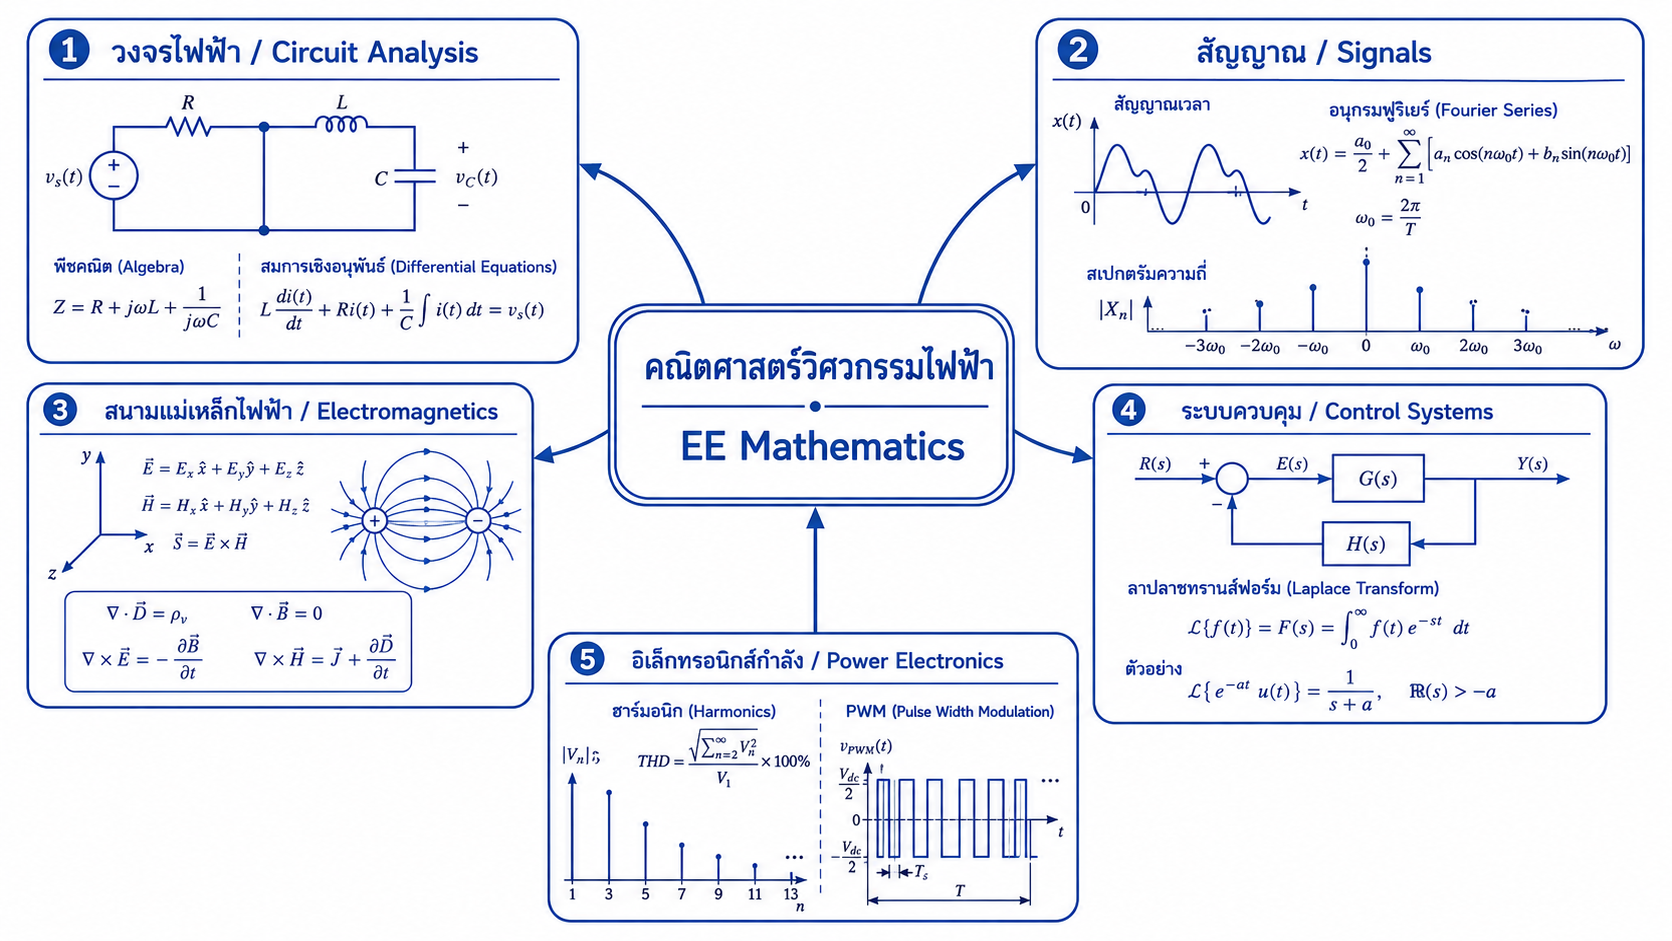
\includegraphics[width=0.8\textwidth]{images/chapter1/figure-01.png}
    \caption{แผนผังความเชื่อมโยงคณิตศาสตร์กับงานวิศวกรรมไฟฟ้า}
\end{figure}

\par\noindent\rule{\textwidth}{0.4pt}\par

\subsection{6. บทนำ}

วิศวกรรมไฟฟ้าเกี่ยวข้องกับการผลิต การส่ง การแปลง การควบคุม และการใช้พลังงานไฟฟ้า ตลอดจนการตรวจวัดและประมวลผลสัญญาณ การออกแบบระบบอิเล็กทรอนิกส์ ระบบควบคุม ระบบสื่อสาร และระบบอัตโนมัติ แม้ระบบเหล่านี้จะมีลักษณะทางกายภาพแตกต่างกัน แต่การวิเคราะห์ล้วนต้องอาศัย “แบบจำลองทางคณิตศาสตร์” เพื่อทำให้ปัญหาที่ซับซ้อนสามารถอธิบายและคำนวณได้

ตัวอย่างเช่น เมื่อพิจารณาวงจรตัวต้านทานอย่างง่าย เราใช้กฎของโอห์มเชื่อมโยงแรงดัน กระแส และความต้านทาน แต่เมื่อวงจรมีตัวเก็บประจุหรือตัวเหนี่ยวนำ ปริมาณไฟฟ้าจะเปลี่ยนแปลงตามเวลาและนำไปสู่สมการเชิงอนุพันธ์ เมื่อวิเคราะห์ไฟฟ้ากระแสสลับ สัญญาณไซน์และมุมเฟสมีบทบาทสำคัญ จึงต้องอาศัยตรีโกณมิติและจำนวนเชิงซ้อน เมื่อศึกษาสนามไฟฟ้าและสนามแม่เหล็ก จำเป็นต้องใช้เวกเตอร์และแคลคูลัสเวกเตอร์ ขณะที่การวิเคราะห์รูปคลื่นที่ไม่เป็นไซน์ต้องอาศัยอนุกรมฟูเรียร์ และการศึกษาการตอบสนองชั่วครู่ของวงจรหรือระบบควบคุมมักใช้การแปลงลาปลาซ

ดังนั้น การเรียนรายวิชานี้จึงไม่ได้มุ่งให้ผู้เรียนจดจำสูตรจำนวนมาก แต่ต้องการให้ผู้เรียนเห็น “ความสัมพันธ์ระหว่างคณิตศาสตร์กับระบบจริง” ตัวอย่างเช่น แรงดันไฟฟ้าบ้านที่ระบุเป็น 220 V ไม่ใช่ค่าสูงสุดของรูปคลื่นไซน์ แต่เป็นค่า RMS ซึ่งสัมพันธ์กับกำลังเฉลี่ยที่จ่ายให้โหลดตัวต้านทาน ความเข้าใจเช่นนี้ช่วยให้ผู้เรียนไม่เพียงคำนวณได้ แต่ยังอธิบายได้ว่าตัวเลขมีความหมายทางกายภาพอย่างไร

ในยุคที่งานวิศวกรรมใช้ซอฟต์แวร์อย่างแพร่หลาย ผู้เรียนต้องรู้ทั้งการคำนวณด้วยมือและการใช้เครื่องมือดิจิทัล การคำนวณด้วยมือทำให้เห็นโครงสร้างของปัญหา ส่วนโปรแกรมช่วยลดงานซ้ำซ้อน เพิ่มความสามารถในการสำรวจค่าพารามิเตอร์ และสร้างกราฟเพื่อมองเห็นพฤติกรรมของระบบ แต่ผลลัพธ์จากโปรแกรมต้องผ่านการตรวจสอบเสมอ โดยเฉพาะเรื่องหน่วย ลำดับขนาด เครื่องหมาย และข้อสมมติของแบบจำลอง

\par\noindent\rule{\textwidth}{0.4pt}\par

\subsection{7. เนื้อหาหลัก}

\subsubsection{7.1 ความสำคัญของคณิตศาสตร์ในงานวิศวกรรมไฟฟ้า}

\paragraph{7.1.1 คณิตศาสตร์ในฐานะภาษาของระบบไฟฟ้า}

ระบบไฟฟ้าประกอบด้วยปริมาณที่สัมพันธ์กันหลายชนิด เช่น แรงดันไฟฟ้า $V$ กระแสไฟฟ้า $I$ ความต้านทาน $R$ กำลังไฟฟ้า $P$ พลังงาน $E$ ความถี่ $f$ และมุมเฟส $\phi$ หากไม่มีสมการ การอธิบายความสัมพันธ์ของปริมาณเหล่านี้จะไม่ชัดเจนและยากต่อการตรวจสอบ

ตัวอย่างพื้นฐานที่สุดคือกฎของโอห์ม

\[
V = IR
\]

\textbf{ที่มา:} เป็นความสัมพันธ์เชิงเส้นขององค์ประกอบตัวต้านทานอุดมคติภายใต้เงื่อนไขที่ค่าความต้านทานคงที่
\textbf{ตัวแปรและหน่วย:} $V$ คือแรงดัน หน่วยโวลต์ (V), $I$ คือกระแส หน่วยแอมแปร์ (A), $R$ คือความต้านทาน หน่วยโอห์ม ($\Omega$)
\textbf{สมมติฐาน:} องค์ประกอบมีพฤติกรรมโอห์มมิกและ $R$ ไม่เปลี่ยนอย่างมีนัยสำคัญจากอุณหภูมิหรือสภาวะอื่น
\textbf{เงื่อนไขการใช้:} ใช้กับตัวต้านทานหรือช่วงการทำงานที่ความสัมพันธ์ $V$–$I$ เป็นเชิงเส้น
\textbf{ความหมายทางกายภาพ:} เมื่อ $R$ คงที่ กระแสเพิ่มตามแรงดันในสัดส่วนเดียวกัน
\textbf{ข้อจำกัด:} อุปกรณ์ไม่เชิงเส้น เช่น ไดโอด ทรานซิสเตอร์ หรือหลอดไฟบางชนิด ไม่สามารถอธิบายด้วย $V=IR$ แบบค่าคงที่เดียวได้ตลอดช่วงการทำงาน

การใช้สมการทำให้สามารถตอบคำถามเชิงวิศวกรรมได้ เช่น หากแรงดันเพิ่มขึ้น 10\% กระแสจะเปลี่ยนอย่างไร หากกำลังของโหลดสูงเกินพิกัดควรปรับความต้านทานเท่าใด หรือหากค่าที่วัดต่างจากแบบจำลอง สาเหตุอาจมาจากความคลาดเคลื่อนของอุปกรณ์หรือไม่

\paragraph{7.1.2 คณิตศาสตร์เพื่อการพยากรณ์และการออกแบบ}

บทบาทของคณิตศาสตร์ในงานวิศวกรรมสามารถแบ่งได้เป็น 4 ระดับ

\begin{enumerate}
    \item \textbf{การบรรยาย (Describe):} ใช้ตัวเลข สมการ และกราฟบอกสถานะของระบบ
    \item \textbf{การวิเคราะห์ (Analyze):} หาความสัมพันธ์ เหตุและผล หรือความไวต่อพารามิเตอร์
    \item \textbf{การพยากรณ์ (Predict):} คำนวณผลที่คาดว่าจะเกิดขึ้นเมื่ออินพุตหรือสภาวะเปลี่ยน
    \item \textbf{การออกแบบ (Design):} เลือกค่าพารามิเตอร์หรือโครงสร้างให้ระบบบรรลุข้อกำหนด
\end{enumerate}

ตัวอย่างเช่น ในวงจรแหล่งจ่ายไฟ วิศวกรอาจเริ่มจากการคำนวณกระแสโหลด ใช้สมการหากำลังสูญเสีย ประเมินอุณหภูมิ และใช้การจำลองตรวจสอบรูปคลื่น ก่อนเลือกอุปกรณ์จริง การคิดเช่นนี้แสดงว่าคณิตศาสตร์เป็นส่วนหนึ่งของวงจรการออกแบบ ไม่ใช่ขั้นตอนแยกต่างหาก

\par\noindent\rule{\textwidth}{0.4pt}\par

\subsubsection{7.2 ความสัมพันธ์ระหว่างคณิตศาสตร์กับวงจรไฟฟ้า สัญญาณ และระบบ}

คณิตศาสตร์แต่ละแขนงมีบทบาทแตกต่างกันตามลักษณะของปัญหา

\begin{table}[htbp]
    \centering
    \begin{tabular}{l l l}
        \hline
        \textbf{งานวิศวกรรมไฟฟ้า} & \textbf{เครื่องมือคณิตศาสตร์หลัก} & \textbf{ตัวอย่างการใช้งาน} \\
        \hline
        วงจรไฟฟ้ากระแสตรง & พีชคณิต สมการเชิงเส้น & หาค่าแรงดัน กระแส กำลัง และการแบ่งแรงดัน \\
        วงจรไฟฟ้ากระแสสลับ & ตรีโกณมิติ จำนวนเชิงซ้อน เฟสเซอร์ & วิเคราะห์ขนาดและมุมเฟสของแรงดัน/กระแส \\
        วงจร RC, RL, RLC ชั่วครู่ & แคลคูลัส สมการเชิงอนุพันธ์ ลาปลาซ & วิเคราะห์การชาร์จ การคายประจุ และการตอบสนองเวลา \\
        สัญญาณไฟฟ้า & ฟังก์ชัน กราฟ ฟูเรียร์ & วิเคราะห์รูปคลื่น ความถี่ และฮาร์มอนิก \\
        สนามไฟฟ้าและสนามแม่เหล็ก & เวกเตอร์ แคลคูลัสเวกเตอร์ & อธิบายขนาด ทิศทาง และการกระจายตัวของสนาม \\
        ระบบควบคุม & สมการเชิงอนุพันธ์ ลาปลาซ ฟังก์ชันถ่ายโอน & วิเคราะห์การตอบสนอง เสถียรภาพ และพฤติกรรมระบบ \\
        ระบบไฟฟ้ากำลัง & จำนวนเชิงซ้อน RMS กำลัง ฮาร์มอนิก & วิเคราะห์กำลัง คุณภาพไฟฟ้า และโหลด AC \\
        อิเล็กทรอนิกส์กำลัง & รูปคลื่น ฟูเรียร์ สมการเชิงอนุพันธ์ & วิเคราะห์ PWM อินเวอร์เตอร์ และฮาร์มอนิก \\
        \hline
    \end{tabular}
\end{table}

ความสัมพันธ์นี้เป็นเหตุผลที่รายวิชาจัดลำดับจากพื้นฐานไปสู่จำนวนเชิงซ้อน เวกเตอร์ ฟูเรียร์ และลาปลาซ ผู้เรียนควรมองแต่ละบทเป็นเครื่องมือใน “กล่องเครื่องมือทางวิศวกรรม” ที่เลือกใช้ตามประเภทของปัญหา

\par\noindent\rule{\textwidth}{0.4pt}\par

\subsubsection{7.3 ภาพรวมเนื้อหาคณิตศาสตร์ที่ใช้ในรายวิชา}

\paragraph{7.3.1 พีชคณิตและการจัดรูปสมการ}

พีชคณิตเป็นพื้นฐานของการแปลงสมการเพื่อหาตัวแปรที่ต้องการ ตัวอย่างจากกฎของโอห์ม

\[
V = IR
\]

สามารถจัดรูปเป็น

\[
I = \frac{V}{R}
\]

และ

\[
R = \frac{V}{I}
\]

การจัดรูปสมการต้องรักษาสมดุลทั้งสองข้างของสมการ ผู้เรียนควรฝึกแยกตัวแปรก่อนแทนค่า เพื่อให้เห็นโครงสร้างและลดความผิดพลาด

\paragraph{7.3.2 ตรีโกณมิติ}

ฟังก์ชันไซน์และโคไซน์ใช้บรรยายสัญญาณเป็นคาบ โดยเฉพาะแรงดันและกระแส AC รูปไซน์ ความสัมพันธ์ของมุม องศา เรเดียน ความถี่ และคาบเวลาจึงเป็นพื้นฐานสำคัญของบทที่ 2 และบทที่ 4–5

\paragraph{7.3.3 จำนวนเชิงซ้อนและเฟสเซอร์}

จำนวนเชิงซ้อนเขียนได้ในรูป

\[
z = a + jb
\]

โดย $a$ เป็นส่วนจริง $b$ เป็นส่วนจินตภาพ และในงานวิศวกรรมไฟฟ้านิยมใช้ $j=\sqrt{-1}$ เพื่อหลีกเลี่ยงความสับสนกับสัญลักษณ์กระแส $i$ จำนวนเชิงซ้อนทำให้การจัดการขนาดและมุมเฟสของสัญญาณไซน์มีประสิทธิภาพมากขึ้น และจะพัฒนาอย่างเป็นระบบในบทที่ 2

\paragraph{7.3.4 เวกเตอร์}

เวกเตอร์ใช้แทนปริมาณที่มีทั้งขนาดและทิศทาง เช่น สนามไฟฟ้า $\mathbf{E}$ หรือสนามแม่เหล็ก $\mathbf{H}$ ตัวอย่างเวกเตอร์ในพิกัดคาร์ทีเซียน

\[
\mathbf{E}=E_x\mathbf{a}_x+E_y\mathbf{a}_y+E_z\mathbf{a}_z
\]

ความหมายขององค์ประกอบและการดำเนินการเวกเตอร์จะเป็นพื้นฐานของการวิเคราะห์สนามในบทที่ 3

\paragraph{7.3.5 แคลคูลัสและสมการเชิงอนุพันธ์}

อนุพันธ์ใช้บอกอัตราการเปลี่ยนแปลง ส่วนปริพันธ์ใช้บอกผลสะสม ตัวอย่างเช่น

\[
i_C(t)=C\frac{dv_C(t)}{dt}
\]

แสดงว่ากระแสผ่านตัวเก็บประจุสัมพันธ์กับอัตราการเปลี่ยนแปลงของแรงดัน การแก้สมการเช่นนี้นำไปสู่รูปเอกซ์โพเนนเชียลและต่อยอดไปสู่การแปลงลาปลาซ

\paragraph{7.3.6 อนุกรมฟูเรียร์}

อนุกรมฟูเรียร์ช่วยแยกรูปคลื่นเป็นคาบที่ไม่ใช่ไซน์บริสุทธิ์ให้เป็นผลรวมขององค์ประกอบไซน์และโคไซน์หลายความถี่ แนวคิดนี้สำคัญต่อการวิเคราะห์ฮาร์มอนิกและคุณภาพกำลังไฟฟ้าในบทที่ 4–5

\paragraph{7.3.7 การแปลงลาปลาซ}

การแปลงลาปลาซช่วยเปลี่ยนปัญหาสมการเชิงอนุพันธ์ในโดเมนเวลาให้เป็นสมการพีชคณิตในโดเมน $s$ ทำให้การวิเคราะห์วงจรชั่วครู่และระบบเชิงเส้นสะดวกขึ้น ซึ่งจะศึกษาในบทที่ 6–7

\par\noindent\rule{\textwidth}{0.4pt}\par

\subsubsection{7.4 หน่วยและสัญลักษณ์พื้นฐานทางวิศวกรรมไฟฟ้า}

\paragraph{7.4.1 เหตุผลที่หน่วยมีความสำคัญ}

คำตอบทางวิศวกรรมที่ไม่มีหน่วยมักไม่สมบูรณ์ เพราะค่าตัวเลขเดียวกันอาจหมายถึงขนาดที่แตกต่างกันอย่างมาก เช่น 5 V, 5 mV และ 5 kV ต่างกันถึงหลายลำดับขนาด การใช้หน่วยอย่างถูกต้องจึงเป็นส่วนหนึ่งของความถูกต้องของสมการ

ตารางต่อไปนี้รวบรวมปริมาณพื้นฐานที่ใช้ในบทนี้

\begin{table}[htbp]
    \centering
    \begin{tabular}{l l l l l}
        \hline
        \textbf{ปริมาณ} & \textbf{สัญลักษณ์ที่ใช้บ่อย} & \textbf{หน่วย} & \textbf{สัญลักษณ์หน่วย} & \textbf{ความหมาย} \\
        \hline
        แรงดันไฟฟ้า & $V$, $v(t)$ & โวลต์ & V & ความต่างศักย์ระหว่างสองจุด \\
        กระแสไฟฟ้า & $I$, $i(t)$ & แอมแปร์ & A & อัตราการไหลของประจุ \\
        ความต้านทาน & $R$ & โอห์ม & $\Omega$ & คุณสมบัติที่ขัดขวางการไหลของกระแส \\
        กำลังไฟฟ้า & $P$, $p(t)$ & วัตต์ & W & อัตราการถ่ายโอนหรือใช้พลังงาน \\
        พลังงาน & $E$ หรือ $W_e$ & จูล & J & พลังงานสะสมหรือพลังงานที่ถ่ายโอน \\
        เวลา & $t$ & วินาที & s & ตัวแปรอิสระของสัญญาณตามเวลา \\
        ความถี่ & $f$ & เฮิรตซ์ & Hz & จำนวนรอบต่อวินาที \\
        คาบเวลา & $T$ & วินาที & s & เวลาครบหนึ่งรอบ \\
        ความถี่เชิงมุม & $\omega$ & เรเดียนต่อวินาที & rad/s & อัตราการเปลี่ยนแปลงมุมเฟส \\
        มุมเฟส & $\phi$ & เรเดียนหรือองศา & rad หรือ $^\circ$ & ตำแหน่งเชิงมุมเทียบกับอ้างอิง \\
        \hline
    \end{tabular}
\end{table}

\paragraph{7.4.2 คำนำหน้าหน่วยที่ใช้บ่อย}

\begin{table}[htbp]
    \centering
    \begin{tabular}{l r r l}
        \hline
        \textbf{คำนำหน้า} & \textbf{สัญลักษณ์} & \textbf{ตัวคูณ} & \textbf{ตัวอย่าง} \\
        \hline
        กิกะ & G & $10^9$ & 1 GHz = $10^9$ Hz \\
        เมกะ & M & $10^6$ & 1 M$\Omega$ = $10^6\ \Omega$ \\
        กิโล & k & $10^3$ & 1 kV = $10^3$ V \\
        มิลลิ & m & $10^{-3}$ & 1 mA = $10^{-3}$ A \\
        ไมโคร & $\mu$ & $10^{-6}$ & 1 $\mu$F = $10^{-6}$ F \\
        นาโน & n & $10^{-9}$ & 1 nF = $10^{-9}$ F \\
        พิโก & p & $10^{-12}$ & 1 pF = $10^{-12}$ F \\
        \hline
    \end{tabular}
\end{table}

\textbf{ข้อควรระวัง:} ตัวพิมพ์ใหญ่และตัวพิมพ์เล็กมีความหมายต่างกัน เช่น m คือ milli แต่ M คือ mega ต่างกัน $10^9$ เท่า จึงต้องรักษารูปแบบสัญลักษณ์อย่างเคร่งครัด

\paragraph{7.4.3 การตรวจสอบมิติของสมการ}

พิจารณาสมการกำลังของโหลดตัวต้านทาน

\[
P=VI
\]

หน่วยของขวามือคือ

\[
\mathrm{V}\cdot\mathrm{A}=\mathrm{W}
\]

ถ้าคำนวณได้ตัวเลขแต่หน่วยไม่สอดคล้องกับวัตต์ แสดงว่าขั้นตอนใดขั้นตอนหนึ่งอาจผิด การตรวจหน่วยจึงเป็นวิธีตรวจความถูกต้องที่รวดเร็ว


\par\noindent\rule{\textwidth}{0.4pt}\par

\subsubsection{7.5 การทบทวนพีชคณิต ฟังก์ชัน กราฟ และสมการพื้นฐาน}

\paragraph{7.5.1 การอ่านสัญลักษณ์ค่าคงที่และฟังก์ชันของเวลา}

ในงานไฟฟ้ามักใช้ตัวพิมพ์ใหญ่แทนค่าคงที่หรือค่าเชิงเฟสเซอร์ และตัวพิมพ์เล็กที่มี $(t)$ แทนค่าทันทีที่เปลี่ยนตามเวลา ตัวอย่างเช่น

\begin{itemize}
    \item $V$ อาจหมายถึงค่าแรงดันคงที่หรือค่า RMS ตามบริบท
    \item $v(t)$ หมายถึงแรงดันทันที ณ เวลา $t$
    \item $I$ อาจหมายถึงกระแสคงที่หรือค่า RMS
    \item $i(t)$ หมายถึงกระแสทันที
\end{itemize}

ผู้เรียนต้องอ่านนิยามของสัญลักษณ์ก่อนใช้สมการทุกครั้ง เพราะสัญลักษณ์เดียวกันอาจมีความหมายต่างกันในเอกสารคนละเล่ม

\paragraph{7.5.2 ฟังก์ชันเชิงเส้น}

รูปทั่วไป

\[
y=mx+b
\]

โดย $m$ คือความชันและ $b$ คือจุดตัดแกน $y$ ความสัมพันธ์ $V=IR$ ของตัวต้านทานที่ $R$ คงที่สามารถมองเป็นเส้นตรงในกราฟ $V$ กับ $I$ โดยความชันเท่ากับ $R$

\paragraph{7.5.3 ฟังก์ชันเอกซ์โพเนนเชียล}

ฟังก์ชันเอกซ์โพเนนเชียลปรากฏบ่อยในวงจรอันดับหนึ่ง เช่น RC และ RL รูปทั่วไปของการเปลี่ยนจากค่าเริ่มต้น $x_i$ ไปสู่ค่าปลายทาง $x_f$ คือ

\[
x(t)=x_f+(x_i-x_f)e^{-t/\tau}
\]

โดย $\tau$ คือค่าคงตัวเวลา เมื่อ $t=\tau$ ส่วนต่างจากค่าปลายทางจะลดเหลือ $e^{-1}\approx0.368$ ของค่าเริ่มต้น และเมื่อประมาณ $5\tau$ ระบบอันดับหนึ่งจะเข้าใกล้ค่าปลายทางมากกว่า 99\% ในเชิงวิศวกรรม

สำหรับวงจร RC

\[
\tau=RC
\]

\textbf{ตัวแปรและหน่วย:} $R$ หน่วยโอห์ม, $C$ หน่วยฟารัด, $\tau$ หน่วยวินาที
\textbf{สมมติฐาน:} $R$ และ $C$ คงที่ วงจรเป็นเชิงเส้น และแหล่งจ่ายเปลี่ยนแบบขั้นบันไดอุดมคติ
\textbf{ความหมายทางกายภาพ:} $\tau$ บอกความเร็วของการตอบสนอง ยิ่ง $RC$ มาก การเปลี่ยนแปลงยิ่งช้า
\textbf{ข้อจำกัด:} อุปกรณ์จริงมีความคลาดเคลื่อนและความต้านทานแฝง จึงอาจทำให้ค่าที่วัดต่างจากแบบจำลอง

% [รูปที่ 2: กราฟการชาร์จและคายประจุของวงจร RC]
% ประเภทภาพ: Graph
% ตำแหน่งที่แนะนำ: หลังหัวข้อ 7.5.3 ฟังก์ชันเอกซ์โพเนนเชียล
% วัตถุประสงค์การเรียนรู้: แสดงความหมายของค่าคงตัวเวลา $\tau$ และพฤติกรรมเข้าใกล้ค่าปลายทางแบบเอกซ์โพเนนเชียล
% คำอธิบายภาพ: แสดงกราฟ normalized voltage เทียบกับเวลา มีเส้น Charging $vC(t)=V0(1-e^{-t/\tau})$ และ Discharging $vC(t)=V0e^{-t/\tau}$ ทำเครื่องหมายที่ $t=\tau$ และ $t=5\tau$ พร้อมค่าประมาณ 0.632 และ 0.368 ที่ $t=\tau$
% องค์ประกอบที่ต้องมี: แกนเวลา $t/\tau$, แกน $vC/V0$, เส้นชาร์จ เส้นคายประจุ เส้นประที่ $\tau$ และ $5\tau$
% ข้อความหรือป้ายกำกับ: “Charging”, “Discharging”, “$t=\tau$”, “$t=5\tau$”, “0.632”, “0.368”
% ภาษาของป้ายกำกับ: อังกฤษและสัญลักษณ์ทางคณิตศาสตร์
% สัดส่วนภาพ: 16:9
% Graph Generation Prompt: Plot normalized RC charging y=1-exp(-t/tau) and discharging y=exp(-t/tau) for t from 0 to 5tau. Horizontal axis labeled t/tau, vertical axis labeled vC/V0. Mark t=tau with charging=0.632 and discharging=0.368, and mark t=5tau. Use clear engineering textbook annotations, white background, readable legend and grid.
% Alt Text: กราฟสองเส้นแสดงแรงดันตัวเก็บประจุขณะชาร์จเพิ่มจากศูนย์เข้าใกล้หนึ่ง และขณะคายประจุลดจากหนึ่งเข้าใกล้ศูนย์ โดยเน้นจุดหนึ่งค่าคงตัวเวลา

\begin{figure}[htbp]
    \centering
    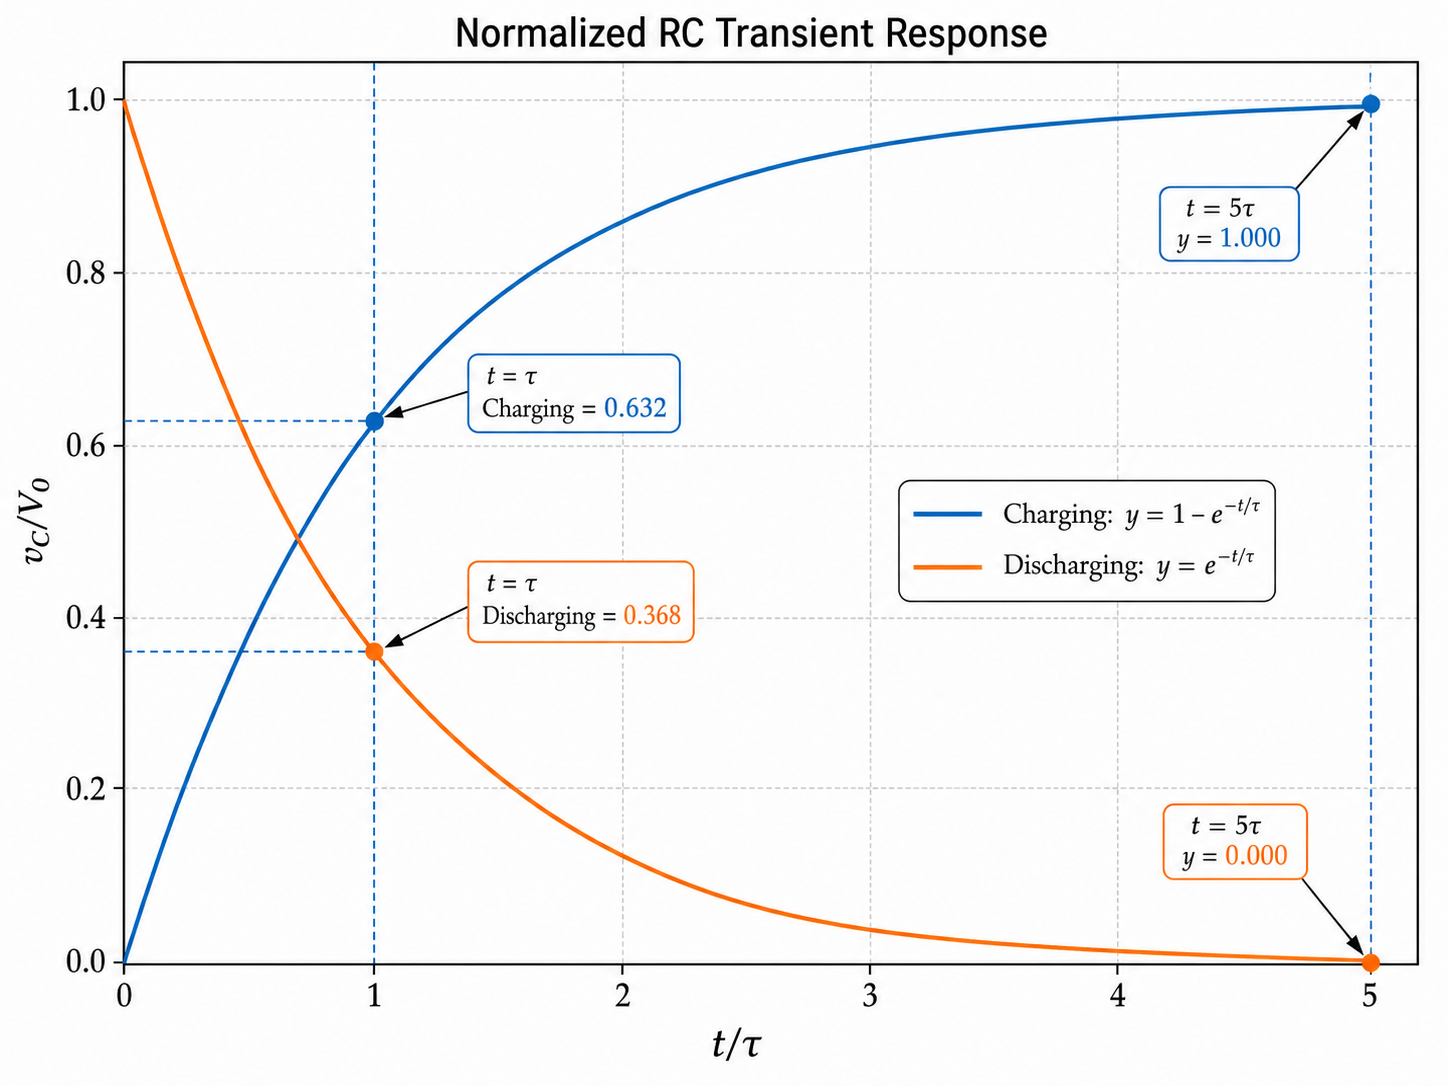
\includegraphics[width=0.8\textwidth]{images/chapter1/figure-02.png}
    \caption{กราฟการชาร์จและคายประจุของวงจร RC}
\end{figure}

\paragraph{7.5.4 ฟังก์ชันไซน์และการแทนสัญญาณ AC}

แรงดันไฟฟ้ากระแสสลับแบบไซน์เขียนได้เป็น

\[
v(t)=V_m\sin(\omega t+\phi)
\]

\textbf{ที่มา:} เป็นแบบจำลองมาตรฐานของสัญญาณฮาร์มอนิกหนึ่งความถี่
\textbf{ตัวแปรและหน่วย:}

\begin{itemize}
    \item $v(t)$ แรงดันทันที หน่วย V
    \item $V_m$ ค่าสูงสุดหรือแอมพลิจูด หน่วย V
    \item $\omega$ ความถี่เชิงมุม หน่วย rad/s
    \item $t$ เวลา หน่วย s
    \item $\phi$ มุมเฟสเริ่มต้น หน่วย rad หรือ $^\circ$
\end{itemize}

\textbf{สมมติฐาน:} สัญญาณเป็นไซน์บริสุทธิ์และพารามิเตอร์คงที่ในช่วงที่วิเคราะห์
\textbf{เงื่อนไขการใช้:} ใช้แทนแรงดันหรือกระแส AC รูปไซน์ และเป็นพื้นฐานของการวิเคราะห์แบบเฟสเซอร์
\textbf{ความหมายทางกายภาพ:} $V_m$ ควบคุมขนาด, $f$ หรือ $\omega$ ควบคุมความเร็วในการวนรอบ, $\phi$ กำหนดการเลื่อนตามแกนเวลา
\textbf{ข้อจำกัด:} รูปคลื่นจากอุปกรณ์สวิตชิ่งหรือโหลดไม่เชิงเส้นอาจไม่ใช่ไซน์บริสุทธิ์และต้องใช้การวิเคราะห์ฮาร์มอนิกเพิ่มเติม

ความสัมพันธ์ระหว่างความถี่ คาบเวลา และความถี่เชิงมุมคือ

\[
T=\frac{1}{f}
\]

และ

\[
\omega=2\pi f=\frac{2\pi}{T}
\]

\textbf{ตัวแปรและหน่วย:} $T$ หน่วย s, $f$ หน่วย Hz, $\omega$ หน่วย rad/s
\textbf{ความหมายทางกายภาพ:} หนึ่งรอบของสัญญาณเท่ากับ $2\pi$ เรเดียน ดังนั้นถ้ามี $f$ รอบต่อวินาที ความเร็วเชิงมุมคือ $2\pi f$ เรเดียนต่อวินาที

\textbf{ตัวอย่างสั้น:} ระบบ 50 Hz มี

\[
T=\frac{1}{50}=0.02\ \mathrm{s}=20\ \mathrm{ms}
\]

และ

\[
\omega=2\pi(50)\approx314.16\ \mathrm{rad/s}
\]

% [รูปที่ 3: กราฟสัญญาณไซน์แสดงพารามิเตอร์สำคัญ]
% ประเภทภาพ: Graph
% ตำแหน่งที่แนะนำ: หลังหัวข้อ 7.5.4 ฟังก์ชันไซน์และการแทนสัญญาณ AC
% วัตถุประสงค์การเรียนรู้: ช่วยให้ผู้เรียนเชื่อมสมการ $v(t)=Vm\sin(\omega t+\phi)$ กับความหมายเชิงกราฟของแอมพลิจูด คาบ และเฟส
% คำอธิบายภาพ: กราฟไซน์หนึ่งถึงสองคาบ แสดงระดับ $+Vm$ และ $-Vm$ ลูกศรค่ายอดถึงยอด $2Vm$ ช่วงคาบ $T$ และการเลื่อนเฟส $\phi$ พร้อมตำแหน่ง zero crossing ที่เหมาะสม
% องค์ประกอบที่ต้องมี: แกน $t$, แกน $v(t)$, เส้นไซน์, เส้นประ $\pm Vm$, ลูกศร $2Vm$, ลูกศร $T$, ตัวบ่งชี้ phase shift
% ข้อความหรือป้ายกำกับ: $Vm$, $-Vm$, $V{pp}=2Vm$, $T=2\pi/\omega$, $\phi$, $v(t)=Vm\sin(\omega t+\phi)$
% ภาษาของป้ายกำกับ: สัญลักษณ์คณิตศาสตร์และอังกฤษสั้น ๆ
% สัดส่วนภาพ: 16:9
% Graph Generation Prompt: Engineering textbook graph of v(t)=Vm sin(omega t + phi) over about two periods. Show horizontal time axis t and vertical voltage axis v(t), dashed levels at +Vm and -Vm, a vertical double arrow labeled Vpp=2Vm, a horizontal arrow labeled T=2pi/omega, and a phase-shift annotation phi. Mark representative zero crossings. White background, clean precise linework, readable mathematical labels, 16:9.
% Alt Text: กราฟไซน์แสดงค่าสูงสุดบวกและลบ ค่ายอดถึงยอด คาบเวลา และการเลื่อนเฟสตามสมการสัญญาณไซน์

\begin{figure}[htbp]
    \centering
    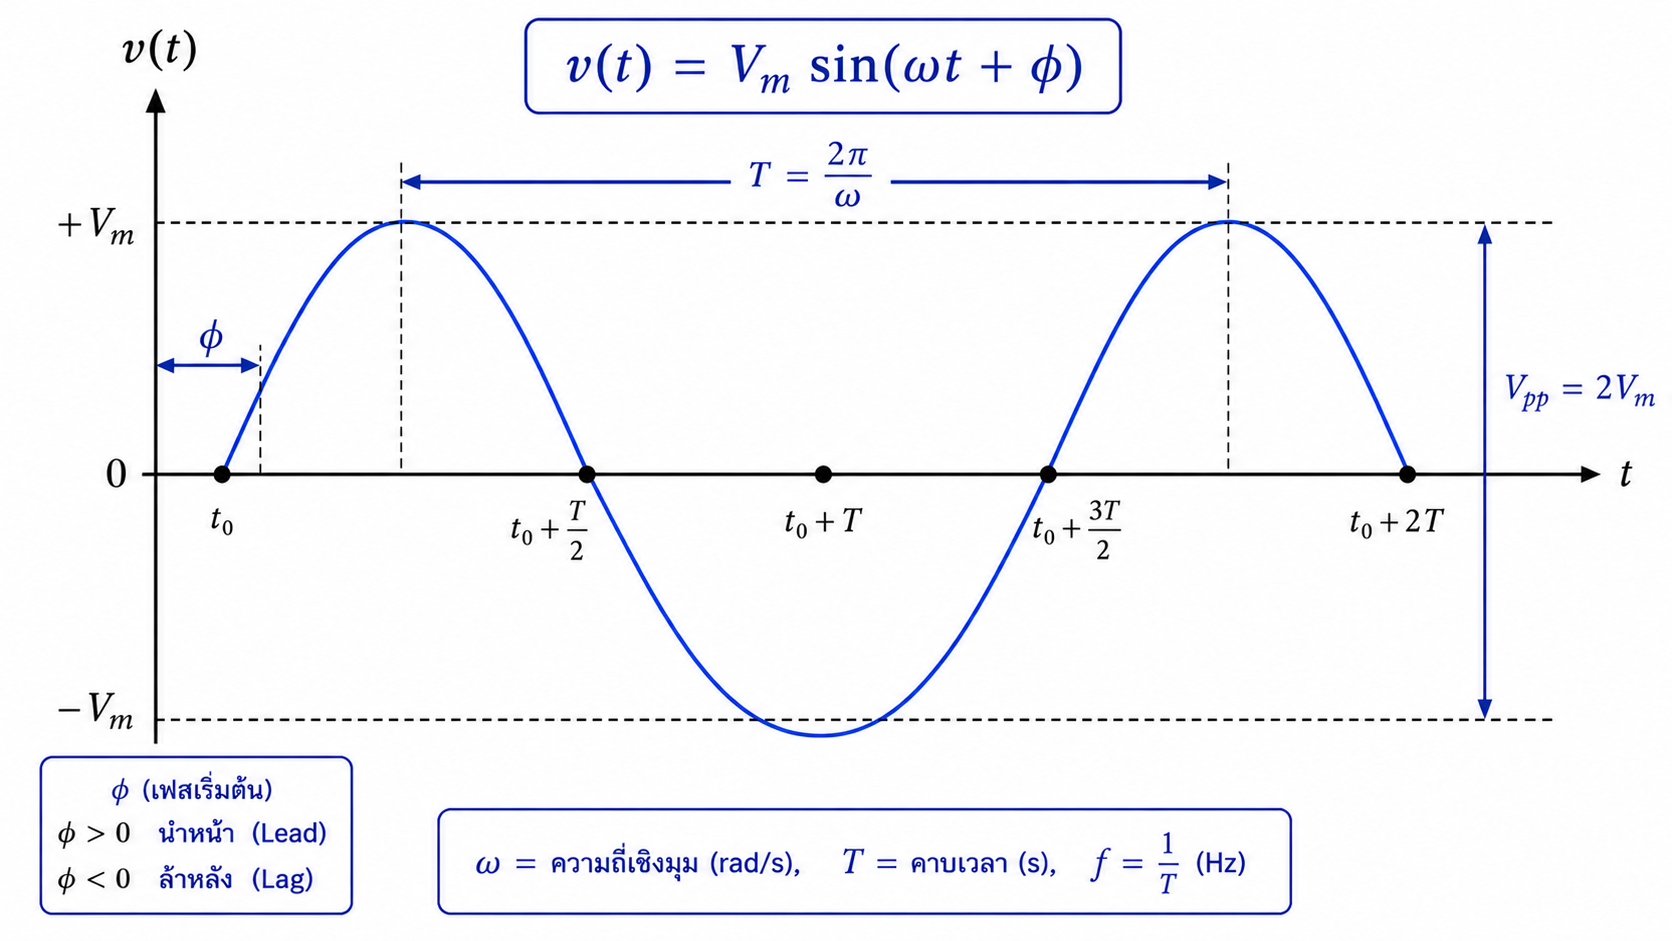
\includegraphics[width=0.8\textwidth]{images/chapter1/figure-03.png}
    \caption{กราฟสัญญาณไซน์แสดงพารามิเตอร์สำคัญ}
\end{figure}

\paragraph{7.5.5 ค่าสูงสุด ค่ายอดถึงยอด ค่าเฉลี่ย และค่า RMS}

สำหรับสัญญาณไซน์สมมาตรรอบศูนย์ ค่าสูงสุดคือ $V_m$ และค่ายอดถึงยอดคือ

\[
V_{pp}=2V_m
\]

ค่าเฉลี่ยทั่วไปของสัญญาณในช่วงหนึ่งคาบนิยามเป็น

\[
V_{\mathrm{avg}}=\frac{1}{T}\int_0^T v(t)\,dt
\]

สำหรับไซน์บริสุทธิ์ตลอดหนึ่งคาบ ค่าเฉลี่ยเท่ากับศูนย์ เพราะพื้นที่บวกและลบหักล้างกัน

\textbf{ข้อสังเกตสำคัญเรื่องค่าเฉลี่ย:} หากพิจารณาเฉพาะครึ่งคาบบวกของไซน์ ค่าเฉลี่ยบนช่วงครึ่งคาบนั้นเท่ากับ $2V_m/\pi$ แต่หากเป็น “สัญญาณครึ่งคลื่นที่ถูกเรียงกระแส” แล้วหาค่าเฉลี่ยตลอดหนึ่งคาบ ค่าเฉลี่ยเท่ากับ $V_m/\pi$ ผู้เรียนต้องระบุช่วงอินทิเกรตให้ชัดเจนเพื่อหลีกเลี่ยงความสับสน

ค่า RMS ของสัญญาณคาบนิยามเป็น

\[
V_{\mathrm{rms}}=\sqrt{\frac{1}{T}\int_0^T v^2(t)\,dt}
\]

สำหรับไซน์บริสุทธิ์

\[
V_{\mathrm{rms}}=\frac{V_m}{\sqrt{2}}\approx0.707V_m
\]

และ

\[
I_{\mathrm{rms}}=\frac{I_m}{\sqrt{2}}\approx0.707I_m
\]

\textbf{ที่มา:} นิยาม RMS มาจากการยกกำลังสอง ค่าเฉลี่ย และถอดราก เพื่อให้ได้ค่าบวกที่สัมพันธ์กับผลของกำลังในโหลดตัวต้านทาน
\textbf{สมมติฐานสำหรับสูตร $V_m/\sqrt{2}$:} รูปคลื่นต้องเป็นไซน์บริสุทธิ์
\textbf{ความหมายทางกายภาพ:} แรงดัน AC ที่มีค่า RMS เท่ากับแรงดัน DC จะให้กำลังเฉลี่ยเท่ากันบนตัวต้านทานเดียวกัน
\textbf{ข้อจำกัด:} สำหรับรูปคลื่นไม่เป็นไซน์ ห้ามใช้ $0.707V_m$ โดยอัตโนมัติ ต้องใช้คำนิยาม RMS หรือวิธีที่เหมาะกับรูปคลื่นนั้น

% [รูปที่ 4: เปรียบเทียบ Peak, Peak-to-Peak และ RMS ของสัญญาณไซน์]
% ประเภทภาพ: Graph
% ตำแหน่งที่แนะนำ: หลังหัวข้อ 7.5.5
% วัตถุประสงค์การเรียนรู้: แยกความหมายของ $Vm$, $V{pp}$ และ $V{rms}$ ซึ่งผู้เรียนมักสับสน
% คำอธิบายภาพ: กราฟไซน์หนึ่งคาบ มีเส้นประระดับ $+Vm$, $-Vm$ และ $+0.707Vm$ พร้อมลูกศรบอก $Vm$ และ $2Vm$
% องค์ประกอบที่ต้องมี: รูปคลื่นไซน์ แกน $t$, แกน $v(t)$ เส้นประ $\pm Vm$, เส้น RMS, ลูกศร $Vm$ และ $V{pp}$
% ข้อความหรือป้ายกำกับ: “Peak $Vm$”, “RMS $=0.707Vm$”, “Peak-to-Peak $=2Vm$”
% ภาษาของป้ายกำกับ: อังกฤษและสัญลักษณ์
% สัดส่วนภาพ: 16:9
% Graph Generation Prompt: Plot one period of a sinusoidal waveform centered at zero. Mark +Vm and -Vm with horizontal dashed lines, mark +0.707Vm as the positive RMS magnitude reference, show a vertical arrow from zero to +Vm labeled Peak Vm, and a vertical double arrow from -Vm to +Vm labeled Peak-to-Peak 2Vm. Include axes v(t) and t, clean engineering textbook style, white background, clear legend.
% Alt Text: กราฟไซน์หนึ่งคาบแสดงความแตกต่างระหว่างค่าสูงสุด ค่ายอดถึงยอด และค่า RMS

\begin{figure}[htbp]
    \centering
    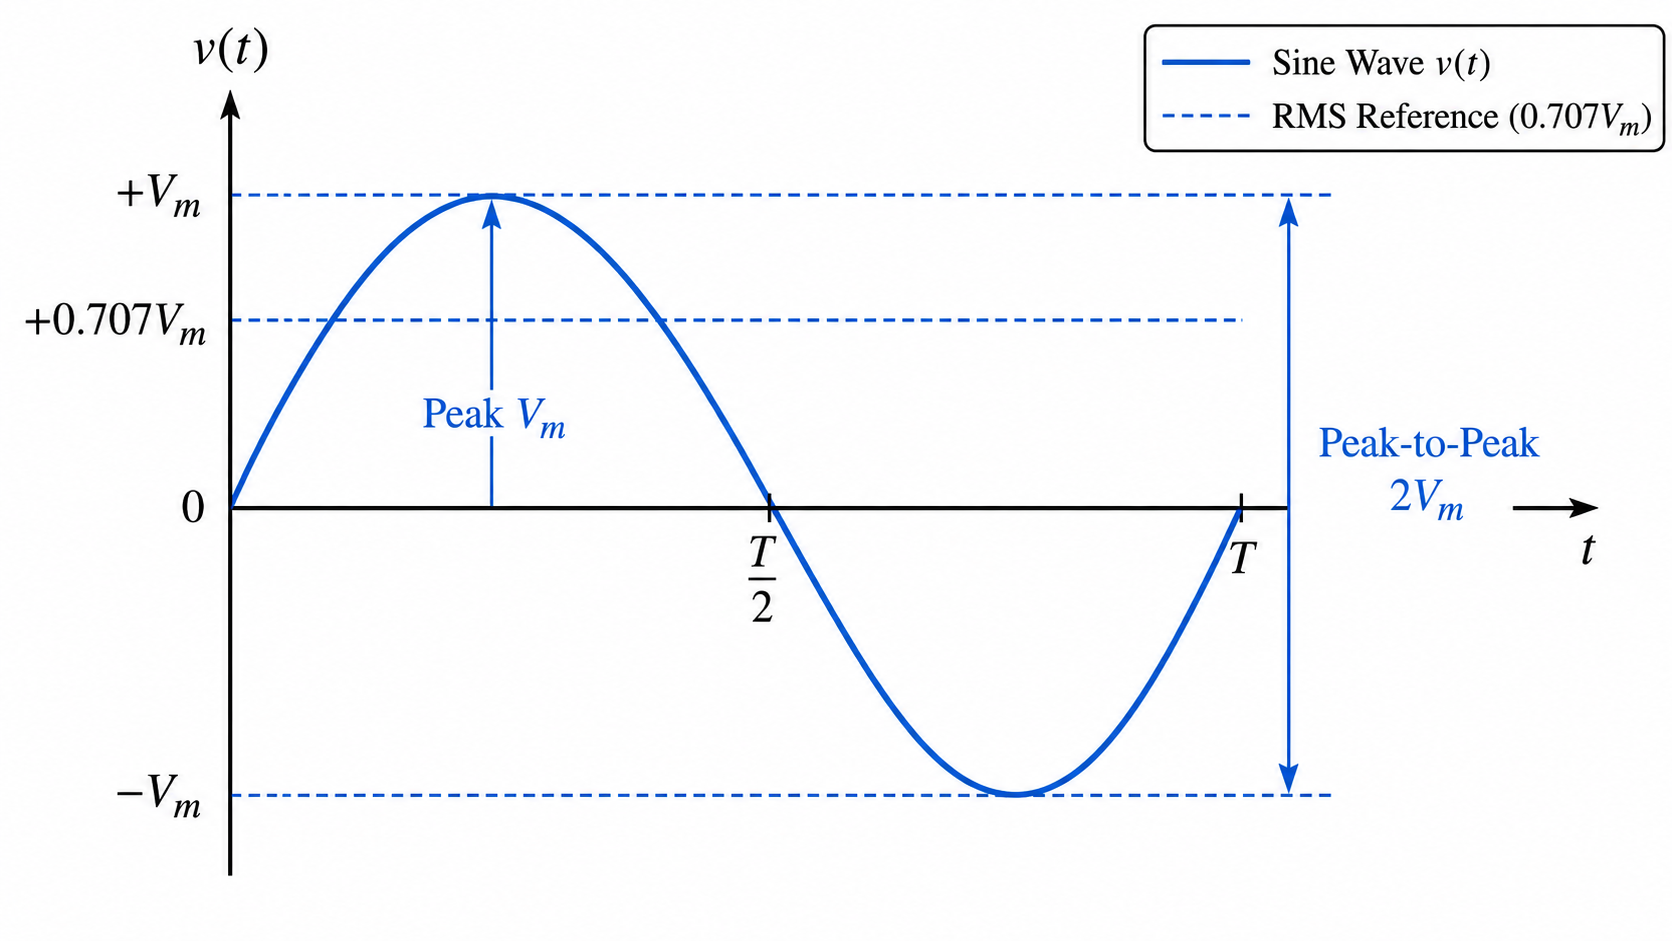
\includegraphics[width=0.8\textwidth]{images/chapter1/figure-04.png}
    \caption{เปรียบเทียบ Peak, Peak-to-Peak และ RMS ของสัญญาณไซน์}
\end{figure}

\paragraph{7.5.6 ความต่างเฟสและการเลื่อนเวลา}

หากสัญญาณสองสัญญาณมีความถี่เท่ากันแต่ต่างเฟสกัน $\Delta\phi$ ความต่างเวลาคำนวณได้จาก

\[
\Delta t=\frac{\Delta\phi}{2\pi f}
\]

เมื่อ $\Delta\phi$ อยู่ในหน่วยเรเดียน หรือ

\[
\Delta t=\left(\frac{\Delta\phi(^\circ)}{360^\circ}\right)T
\]

เมื่อมุมอยู่ในหน่วยองศา

\textbf{เงื่อนไขการใช้:} สัญญาณต้องมีความถี่เดียวกัน
\textbf{ความหมายทางกายภาพ:} มุมเฟสคือการบอกตำแหน่งในรอบ ถ้าหนึ่งรอบใช้เวลา $T$ การเหลื่อม $30^\circ$ จึงเท่ากับ $30/360$ ของคาบ
\textbf{ข้อควรระวัง:} เครื่องหมายของ $\Delta t$ ขึ้นกับนิยามว่าสัญญาณใดเป็นตัวอ้างอิงและใช้คำว่า “นำ” หรือ “ล้า”

\paragraph{7.5.7 สัญญาณรูปแบบอื่นที่ควรรู้จัก}

แม้บทนี้เน้นสัญญาณไซน์ ผู้เรียนควรรู้จักรูปคลื่นพื้นฐานอื่นเพื่อเตรียมพร้อมสำหรับบทต่อไป

\begin{itemize}
    \item \textbf{สัญญาณขั้นบันได (Unit Step):} ใช้แทนการเปลี่ยนสถานะทันที เช่น การเปิดสวิตช์
    \item \textbf{สัญญาณเอกซ์โพเนนเชียล:} พบในการตอบสนองชั่วครู่ของวงจร RC และ RL
    \item \textbf{สัญญาณสี่เหลี่ยม:} พบในวงจรดิจิทัลและ PWM มีฮาร์มอนิกหลายอันดับ
    \item \textbf{สัญญาณสามเหลี่ยมและฟันเลื่อย:} พบในการสร้างสัญญาณ การมอดูเลต และวงจรควบคุมบางประเภท
\end{itemize}

รูปคลื่นที่ไม่เป็นไซน์บริสุทธิ์จะเชื่อมโยงโดยตรงกับอนุกรมฟูเรียร์ในบทที่ 4 และการวิเคราะห์รูปคลื่นไฟฟ้าในบทที่ 5

\par\noindent\rule{\textwidth}{0.4pt}\par

\subsubsection{7.6 การคำนวณเชิงตัวเลขและการประมาณค่า}

\paragraph{7.6.1 สัญกรณ์วิทยาศาสตร์และสัญกรณ์วิศวกรรม}

การเขียนตัวเลขขนาดใหญ่มากหรือเล็กมากในรูป

\[
a\times10^n
\]

ช่วยให้คำนวณและเปรียบเทียบลำดับขนาดได้ง่าย ในสัญกรณ์วิศวกรรม มักเลือกเลขชี้กำลังเป็นพหุคูณของ 3 เพื่อให้สัมพันธ์กับคำนำหน้าหน่วย เช่น

\[
0.0000047\ \mathrm{F}=4.7\times10^{-6}\ \mathrm{F}=4.7\ \mu\mathrm{F}
\]

และ

\[
4700\ \Omega=4.7\times10^3\ \Omega=4.7\ \mathrm{k}\Omega
\]

\paragraph{7.6.2 เลขนัยสำคัญ}

เลขนัยสำคัญสะท้อนความละเอียดของข้อมูล ตัวอย่างเช่น หากตัวต้านทานระบุ $100\ \Omega$ ด้วยความคลาดเคลื่อน 5\% การรายงานผลคำนวณเป็น $99.999873\ \Omega$ ไม่มีความหมายทางกายภาพมากกว่าการรายงานอย่างเหมาะสมตามความละเอียดของข้อมูล

แนวปฏิบัติพื้นฐานคือ

\begin{itemize}
    \item เก็บจำนวนหลักมากพอในระหว่างการคำนวณ
    \item ปัดเศษในขั้นตอนสุดท้าย
    \item ไม่รายงานทศนิยมมากเกินความแม่นของข้อมูลนำเข้า
    \item ระบุหน่วยทุกครั้ง
\end{itemize}

\paragraph{7.6.3 ความคลาดเคลื่อนสัมบูรณ์และความคลาดเคลื่อนสัมพัทธ์}

ให้ $x_{ref}$ เป็นค่าอ้างอิง และ $x_{approx}$ เป็นค่าประมาณ

\[
E_{abs}=|x_{ref}-x_{approx}|
\]

ความคลาดเคลื่อนสัมพัทธ์คือ

\[
E_{rel}=\frac{|x_{ref}-x_{approx}|}{|x_{ref}|}
\]

และร้อยละความคลาดเคลื่อนคือ

\[
E_{\%}=E_{rel}\times100\%
\]

\textbf{ข้อจำกัด:} หาก $x_{ref}=0$ ไม่สามารถใช้สูตรความคลาดเคลื่อนสัมพัทธ์แบบนี้ได้โดยตรง

\paragraph{7.6.4 การประมาณค่าเพื่อทดสอบความสมเหตุสมผล}

ก่อนกดเครื่องคิดเลขควรถามว่า “คำตอบควรอยู่ประมาณเท่าใด” ตัวอย่างเช่น $220^2/100$ ควรมีค่าประมาณ $484$ ไม่ใช่ $48{,}400$ หรือ $4.84$ การประมาณลำดับขนาดช่วยจับข้อผิดพลาดเรื่องจุดทศนิยม คำนำหน้าหน่วย และการพิมพ์สูตรผิด

\textbf{ตัวอย่าง:} ถ้าโหลด $R=100\ \Omega$ ต่อกับ $V_{rms}=220\ \mathrm{V}$

\[
P=\frac{V_{rms}^2}{R}\approx\frac{(2.2\times10^2)^2}{10^2}\approx4.84\times10^2\ \mathrm{W}
\]

ดังนั้นคำตอบควรอยู่ระดับหลายร้อยวัตต์

\paragraph{7.6.5 ความผิดพลาดเชิงตัวเลขที่พบบ่อย}

\begin{enumerate}
    \item ใช้องศาแทนเรเดียนหรือกลับกัน
    \item พิมพ์วงเล็บไม่ครบ เช่น $1/2\pi f$ แทน $1/(2\pi f)$
    \item ลืมแปลง mA เป็น A ก่อนคำนวณกำลัง
    \item ปัดเศษเร็วเกินไปจนเกิดความคลาดเคลื่อนสะสม
    \item ใช้ค่าคงที่ $\pi\approx3.14$ ในขั้นตอนกลางมากเกินจำเป็น
    \item เชื่อผลเครื่องคิดเลขโดยไม่ตรวจลำดับขนาด
\end{enumerate}

\par\noindent\rule{\textwidth}{0.4pt}\par

\subsubsection{7.7 เครื่องมือคำนวณทางคณิตศาสตร์สำหรับวิศวกรรมไฟฟ้า}

เครื่องมือคำนวณช่วยให้ผู้เรียนทดลองกับปัญหาที่มีข้อมูลจำนวนมากหรือแสดงผลเป็นกราฟได้สะดวก แต่การเลือกเครื่องมือควรสัมพันธ์กับวัตถุประสงค์

\begin{table}[htbp]
    \centering
    \begin{tabular}{l l l l}
        \hline
        \textbf{เครื่องมือ} & \textbf{จุดเด่น} & \textbf{การใช้งานที่เหมาะสมในรายวิชา} & \textbf{ข้อสังเกต} \\
        \hline
        เครื่องคิดเลขวิทยาศาสตร์ & รวดเร็ว พกพา ใช้งานออฟไลน์ & คำนวณพื้นฐาน จำนวนเชิงซ้อน ตรีโกณมิติ & ต้องตรวจโหมด DEG/RAD \\
        Python & ภาษาทั่วไป ใช้งานได้กว้าง มีระบบนิเวศวิทยาศาสตร์ & คำนวณ สร้างกราฟ วิเคราะห์ข้อมูล และเขียนสคริปต์ & ต้องติดตั้งไลบรารีหรือใช้ Notebook ออนไลน์ \\
        NumPy & อาร์เรย์และการคำนวณเชิงตัวเลข & เวกเตอร์ เมทริกซ์ ฟังก์ชันตรีโกณมิติ & เน้นการคำนวณเชิงตัวเลข \\
        Matplotlib & การสร้างภาพและกราฟ & รูปคลื่นแรงดัน กระแส และผลการจำลอง & ต้องกำหนดแกน หน่วย และคำอธิบายให้ชัด \\
        SciPy & อัลกอริทึมวิทยาศาสตร์และวิศวกรรม & อินทิเกรต ระบบสัญญาณ การเพิ่มประสิทธิภาพ & เหมาะกับงานที่ซับซ้อนกว่าพื้นฐาน \\
        SymPy & คำนวณเชิงสัญลักษณ์ & จัดรูปสมการ อนุพันธ์ ปริพันธ์ และตรวจสมการ & ผลเชิงสัญลักษณ์ต้องตีความร่วมกับสมมติฐาน \\
        MATLAB & สภาพแวดล้อมคำนวณเชิงตัวเลขและกราฟสำหรับวิศวกรรม & เมทริกซ์ สัญญาณ การควบคุม และการจำลอง & สิทธิ์ใช้งานขึ้นกับสถาบัน \\
        GNU Octave & ซอฟต์แวร์เสรีที่มีไวยากรณ์ใกล้ MATLAB ในงานจำนวนมาก & งานคำนวณเมทริกซ์และกราฟพื้นฐาน & ความเข้ากันได้ไม่สมบูรณ์ทุกกรณี \\
        Google Colab & Notebook แบบโฮสต์ ใช้ผ่านเว็บโดยไม่ต้องตั้งค่าท้องถิ่น & ทดลอง Python แชร์งาน และเรียนแบบปฏิบัติ & ทรัพยากรและข้อจำกัดการใช้งานอาจเปลี่ยนแปลง \\
        GeoGebra หรือเครื่องมือกราฟออนไลน์ & สร้างกราฟแบบโต้ตอบ & สำรวจฟังก์ชันและพารามิเตอร์ & ไม่ทดแทนการคำนวณเชิงวิศวกรรมเต็มรูปแบบ \\
        \hline
    \end{tabular}
\end{table}

\paragraph{7.7.1 หลักการใช้ซอฟต์แวร์อย่างมีวิจารณญาณ}

ก่อนใช้โปรแกรม ผู้เรียนควรตอบคำถาม 5 ข้อ

\begin{enumerate}
    \item อินพุตคืออะไร และมีหน่วยอะไร
    \item สมการหรือแบบจำลองที่โปรแกรมกำลังคำนวณคืออะไร
    \item พารามิเตอร์แต่ละตัวมีช่วงค่าที่สมเหตุสมผลหรือไม่
    \item ผลลัพธ์คาดว่าจะมีลำดับขนาดประมาณใด
    \item จะตรวจสอบผลด้วยวิธีอื่นอย่างไร เช่น คำนวณด้วยมือ กรณีพิเศษ หรือการตรวจหน่วย
\end{enumerate}

\paragraph{7.7.2 ตัวอย่างโปรแกรม Python: วาดรูปคลื่นแรงดัน AC}

ตัวอย่างต่อไปใช้ NumPy สำหรับสร้างข้อมูลเวลาและคำนวณฟังก์ชันไซน์ และใช้ Matplotlib สำหรับสร้างกราฟ

\begin{verbatim}
import numpy as np
import matplotlib.pyplot as plt

# พารามิเตอร์ของสัญญาณ
Vm = 311.0          # V
f = 50.0            # Hz
omega = 2 * np.pi * f
phi = 0.0           # rad

# สร้างแกนเวลา 0–40 ms ครอบคลุม 2 คาบของระบบ 50 Hz
t = np.linspace(0.0, 0.040, 1000)

# คำนวณแรงดันตามเวลา
v = Vm * np.sin(omega * t + phi)
Vrms = Vm / np.sqrt(2)

# วาดกราฟ
plt.figure(figsize=(10, 4))
plt.plot(t * 1000, v, label="v(t)")
plt.axhline(Vm, linestyle="--", label=f"Peak = {Vm:.0f} V")
plt.axhline(Vrms, linestyle="-.", label=f"RMS = {Vrms:.1f} V")
plt.xlabel("Time (ms)")
plt.ylabel("Voltage (V)")
plt.title("Sinusoidal voltage: v(t) = 311 sin(2π50t)")
plt.grid(True)
plt.legend()
plt.tight_layout()
plt.show()
\end{verbatim}

\textbf{การอธิบายโค้ดเป็นส่วน ๆ}

\begin{itemize}
    \item \texttt{np.linspace} สร้างจุดเวลาจำนวน 1,000 จุดในช่วง 0–0.040 s
    \item \texttt{omega = 2*np.pi*f} คำนวณความถี่เชิงมุม
    \item \texttt{np.sin} คำนวณค่าไซน์แบบเวกเตอร์สำหรับทุกจุดเวลา
    \item \texttt{Vrms = Vm/np.sqrt(2)} ใช้ได้เพราะกำหนดให้สัญญาณเป็นไซน์บริสุทธิ์
    \item การคูณ \texttt{t*1000} เปลี่ยนหน่วยแกนเวลาเป็นมิลลิวินาทีเพื่ออ่านกราฟง่ายขึ้น
\end{itemize}

\textbf{ผลลัพธ์ที่ควรสังเกต:} ค่าสูงสุดประมาณ 311 V, คาบประมาณ 20 ms และค่า RMS ประมาณ 219.9 V

\textbf{การตรวจสอบผล:} คำนวณด้วยมือว่า $T=1/50=20$ ms และ $311/\sqrt{2}\approx219.9$ V แล้วเปรียบเทียบกับกราฟ

% [รูปที่ 5: ผลลัพธ์กราฟแรงดัน AC จากโปรแกรม Python/Matplotlib]
% ประเภทภาพ: Graph
% ตำแหน่งที่แนะนำ: หลังตัวอย่างโปรแกรม Python ในหัวข้อ 7.7.2
% วัตถุประสงค์การเรียนรู้: เชื่อมโค้ดกับผลลัพธ์ทางกายภาพของสัญญาณ 50 Hz
% คำอธิบายภาพ: กราฟ $v(t)=311\sin(2\pi50t)$ ตั้งแต่ 0 ถึง 40 ms แสดงสองคาบ มีเส้นอ้างอิง Peak 311 V และ RMS ประมาณ 220 V
% องค์ประกอบที่ต้องมี: แกนเวลา ms แกนแรงดัน V รูปคลื่นไซน์ เส้น Peak เส้น RMS legend และ grid
% ข้อความหรือป้ายกำกับ: “Peak = 311 V”, “RMS ≈ 220 V”, “T = 20 ms”
% ภาษาของป้ายกำกับ: อังกฤษหรือไทยและอังกฤษ
% สัดส่วนภาพ: 16:9
% Graph Generation Prompt: Plot v(t)=311sin(2pi50t) for t from 0 to 0.04 seconds, display time in milliseconds and voltage in volts. Show two periods, add horizontal reference lines for Peak=311 V and RMS=311/sqrt(2)≈220 V, and annotate T=20 ms. Include title, axes with units, legend, and grid. Clean engineering textbook graph.
% Alt Text: กราฟแรงดันไซน์ 50 เฮิรตซ์สองคาบ แสดงค่าสูงสุด 311 โวลต์ ค่า RMS ประมาณ 220 โวลต์ และคาบ 20 มิลลิวินาที

\begin{figure}[htbp]
    \centering
    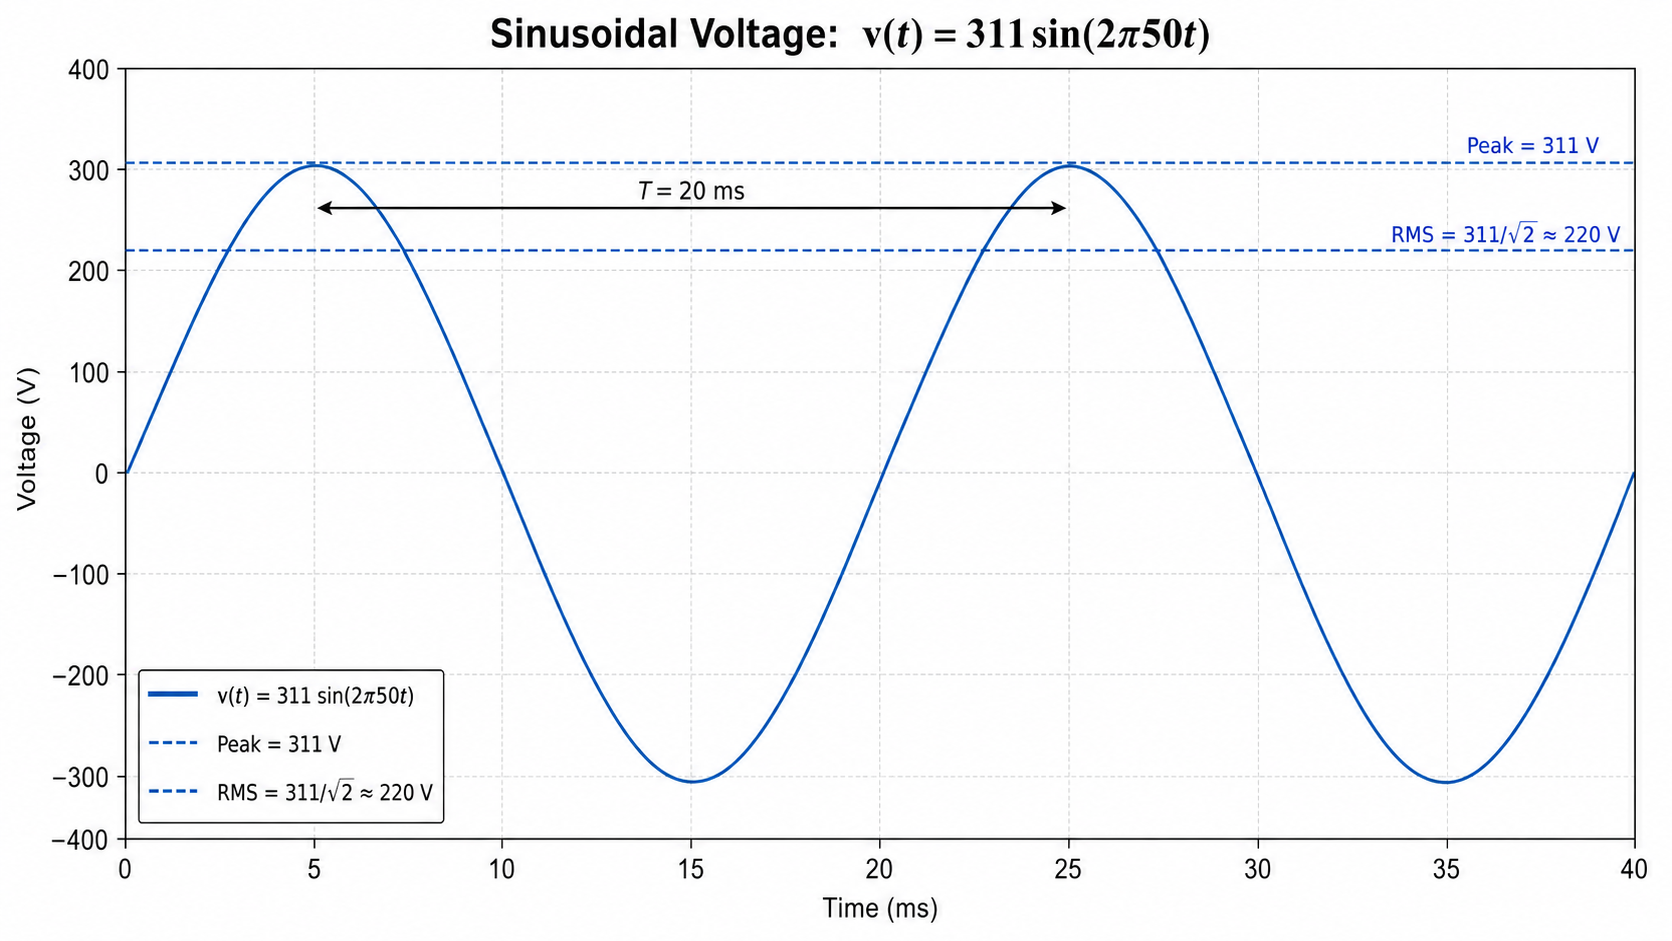
\includegraphics[width=0.8\textwidth]{images/chapter1/figure-05.png}
    \caption{ผลลัพธ์กราฟแรงดัน AC จากโปรแกรม Python/Matplotlib}
\end{figure}

\par\noindent\rule{\textwidth}{0.4pt}\par

\subsubsection{7.8 แนวทางการแก้ปัญหาทางคณิตศาสตร์ในงานวิศวกรรมไฟฟ้า}

การแก้โจทย์อย่างเป็นระบบสำคัญกว่าการจำสูตร กระบวนการแนะนำมี 9 ขั้นตอน

\paragraph{ขั้นที่ 1 ทำความเข้าใจระบบและคำถาม}

ระบุว่าโจทย์ต้องการหาอะไร ระบบเป็น DC หรือ AC สัญญาณคงที่หรือเปลี่ยนตามเวลา และมีองค์ประกอบใดบ้าง

\paragraph{ขั้นที่ 2 กำหนดตัวแปร อ้างอิง และหน่วย}

เขียนสัญลักษณ์ของค่าที่ทราบและค่าที่ไม่ทราบ แปลงหน่วยให้อยู่ในระบบที่สอดคล้องกัน เช่น mA เป็น A ก่อนแทนในสูตรกำลัง

\paragraph{ขั้นที่ 3 วาดภาพหรือแบบจำลองอย่างง่าย}

วงจร แผนภาพบล็อก หรือกราฟช่วยลดความคลุมเครือ โดยเฉพาะเรื่องทิศทางกระแส ขั้วแรงดัน และการนำ–ล้าของเฟส

\paragraph{ขั้นที่ 4 เลือกหลักการหรือกฎ}

เลือกกฎของโอห์ม กำลังไฟฟ้า สมการไซน์ ความสัมพันธ์ $f$–$T$–$\omega$ หรือหลักการอื่นให้ตรงกับปัญหา

\paragraph{ขั้นที่ 5 สร้างสมการก่อนแทนค่า}

เขียนสมการเชิงสัญลักษณ์เพื่อเห็นความสัมพันธ์ จากนั้นจัดรูปให้ตัวแปรที่ต้องการอยู่ด้านเดียว

\paragraph{ขั้นที่ 6 แทนค่าและคำนวณ}

แทนค่าพร้อมหน่วย ควบคุมวงเล็บและโหมดเครื่องคิดเลขให้ถูกต้อง

\paragraph{ขั้นที่ 7 ตรวจสอบหน่วยและมิติ}

ตรวจว่าหน่วยสุดท้ายตรงกับปริมาณที่ต้องการ เช่น กำลังต้องเป็นวัตต์

\paragraph{ขั้นที่ 8 ตรวจสอบความสมเหตุสมผล}

ถามว่าคำตอบมีเครื่องหมายและลำดับขนาดสมเหตุสมผลหรือไม่ ถ้าแรงดันเพิ่มแต่ผลคำนวณกระแสลดทั้งที่ $R$ คงที่ อาจมีข้อผิดพลาด

\paragraph{ขั้นที่ 9 แปลความหมายทางวิศวกรรม}

คำตอบไม่ควรจบเพียงตัวเลข แต่ควรบอกว่าผลนั้นหมายถึงอะไร เช่น โหลดใช้กำลัง 484 W หรือสัญญาณที่สองนำสัญญาณแรก 1.67 ms

% [รูปที่ 6: กระบวนการแก้ปัญหาคณิตศาสตร์สำหรับงานวิศวกรรมไฟฟ้า]
% ประเภทภาพ: Flowchart
% ตำแหน่งที่แนะนำ: หลังหัวข้อ 7.8
% วัตถุประสงค์การเรียนรู้: ทำให้ผู้เรียนมีขั้นตอนมาตรฐานในการแก้ปัญหาและตรวจสอบคำตอบ
% คำอธิบายภาพ: Flowchart จาก “Understand Problem” → “Define Variables & Units” → “Draw Model” → “Select Principle” → “Form Equation” → “Substitute & Calculate” → “Check Units” → “Check Reasonableness” → “Interpret Engineering Meaning” และมีลูกศรย้อนกลับจากขั้นตรวจสอบหากผลไม่สมเหตุสมผล
% องค์ประกอบที่ต้องมี: กล่อง 9 ขั้น ลูกศรตามลำดับ ลูกศร feedback จาก Check ไปยัง Select Principle/Form Equation
% ข้อความหรือป้ายกำกับ: ไทยและอังกฤษแบบสั้น
% ภาษาของป้ายกำกับ: ไทยและอังกฤษ
% สัดส่วนภาพ: 16:9
% Image Generation Prompt: Clean engineering education flowchart with nine steps: Understand Problem → Define Variables & Units → Draw Model → Select Principle → Form Equation → Substitute & Calculate → Check Units → Check Reasonableness → Interpret Engineering Meaning. Add feedback arrows from both checking steps back to model/equation selection when an inconsistency is found. White background, precise arrows, minimal blue technical style, bilingual Thai-English labels, 16:9.
% Alt Text: ผังงานเก้าขั้นตอนสำหรับแก้ปัญหาทางวิศวกรรม ตั้งแต่ทำความเข้าใจโจทย์จนถึงแปลความหมายคำตอบ พร้อมวงรอบย้อนกลับเมื่อตรวจพบความไม่สอดคล้อง

\begin{figure}[htbp]
    \centering
    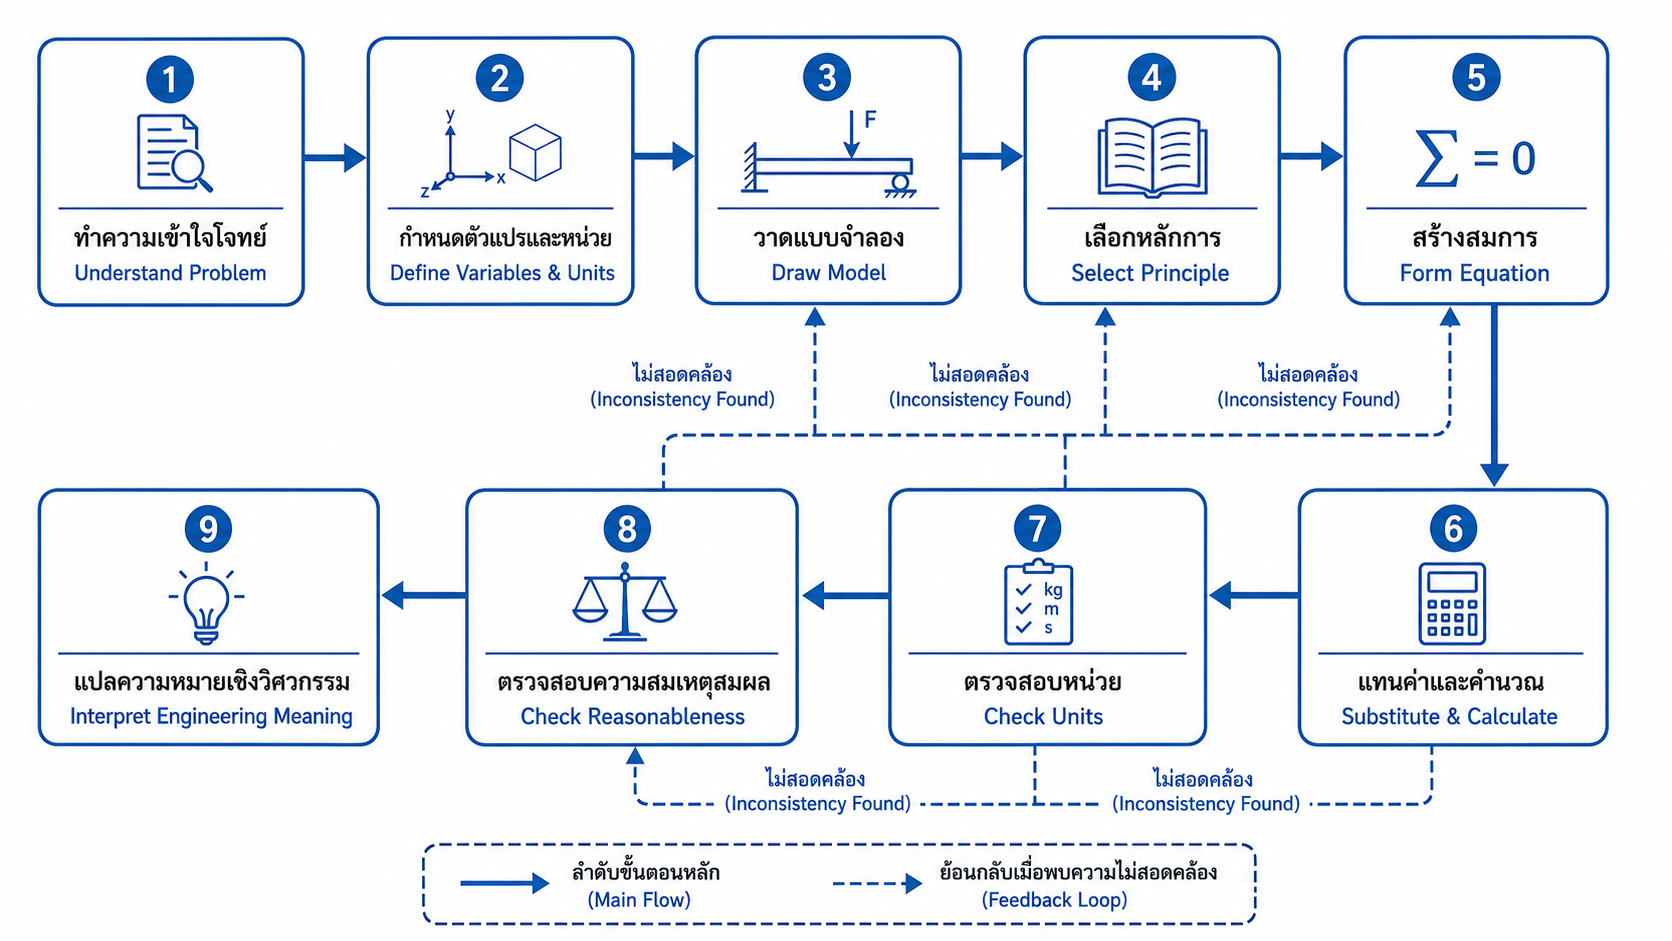
\includegraphics[width=0.8\textwidth]{images/chapter1/figure-06.png}
    \caption{กระบวนการแก้ปัญหาคณิตศาสตร์สำหรับงานวิศวกรรมไฟฟ้า}
\end{figure}


\par\noindent\rule{\textwidth}{0.4pt}\par

\subsubsection{7.9 ตัวอย่างโจทย์พื้นฐานที่เชื่อมโยงกับวงจรไฟฟ้า}

\paragraph{ตัวอย่างที่ 1.1 การใช้กฎของโอห์มและการตรวจหน่วย}

\textbf{โจทย์:} ตัวต้านทาน $R=47\ \Omega$ ต่อกับแหล่งจ่าย DC $V=12\ \mathrm{V}$ จงหากระแสที่ไหลและกำลังที่ตัวต้านทาน

\textbf{1) วิเคราะห์ระบบหรือโจทย์}
เป็นวงจร DC ตัวต้านทานอุดมคติ ต้องการ $I$ และ $P$

\textbf{2) กำหนดตัวแปรและหน่วย}
$V=12\ \mathrm{V}$, $R=47\ \Omega$

\textbf{3) เลือกกฎหรือหลักการ}
ใช้กฎของโอห์มและสูตรกำลัง

\[
I=\frac{V}{R}
\]

\[
P=VI
\]

\textbf{4) แทนค่าและคำนวณ}

\[
I=\frac{12}{47}=0.2553\ \mathrm{A}
\]

ประมาณ

\[
I\approx0.255\ \mathrm{A}=255\ \mathrm{mA}
\]

กำลัง

\[
P=(12)(0.2553)\approx3.06\ \mathrm{W}
\]

\textbf{5) ตรวจสอบหน่วย}
$\mathrm{V}/\Omega=\mathrm{A}$ และ $\mathrm{V}\cdot\mathrm{A}=\mathrm{W}$ ถูกต้อง

\textbf{6) ตรวจสอบความสมเหตุสมผล}
$12/50\approx0.24$ A ดังนั้น 0.255 A สมเหตุสมผล

\textbf{7) แปลความหมาย}
ตัวต้านทานต้องรับกำลังประมาณ 3.06 W ในแบบจำลองอุดมคติ การเลือกตัวต้านทานจริงต้องพิจารณาพิกัดกำลังและการระบายความร้อนเพิ่มเติม

\par\noindent\rule{\textwidth}{0.4pt}\par

\paragraph{ตัวอย่างที่ 1.2 การคำนวณพารามิเตอร์ของแรงดัน AC}

\textbf{โจทย์:} กำหนด

\[
v(t)=311\sin(314t)\ \mathrm{V}
\]

จงหา (ก) ค่าสูงสุด (ข) ค่า RMS (ค) ความถี่ (ง) คาบเวลา

\textbf{1) วิเคราะห์รูปมาตรฐาน}

เปรียบเทียบกับ

\[
v(t)=V_m\sin(\omega t+\phi)
\]

ได้ $V_m=311$ V, $\omega=314$ rad/s และ $\phi=0$

\textbf{2) ค่าสูงสุด}

\[
V_m=311\ \mathrm{V}
\]

\textbf{3) ค่า RMS}

\[
V_{rms}=\frac{311}{\sqrt{2}}\approx219.9\ \mathrm{V}
\]

\textbf{4) ความถี่}

\[
f=\frac{\omega}{2\pi}=\frac{314}{2\pi}\approx49.97\ \mathrm{Hz}
\]

โดยมักประมาณเป็น 50 Hz

\textbf{5) คาบเวลา}

\[
T=\frac{1}{f}\approx\frac{1}{49.97}\approx0.0200\ \mathrm{s}=20.0\ \mathrm{ms}
\]

\textbf{6) ตรวจสอบ}
ถ้า $f\approx50$ Hz คาบควรประมาณ 20 ms จึงสอดคล้องกัน

\textbf{คำตอบ:} $V_m=311$ V, $V_{rms}\approx219.9$ V, $f\approx50$ Hz และ $T\approx20$ ms

\par\noindent\rule{\textwidth}{0.4pt}\par

\paragraph{ตัวอย่างที่ 1.3 การหาสมการแรงดันจากค่า RMS}

\textbf{โจทย์:} ระบบ AC มี $V_{rms}=220\ \mathrm{V}$, $f=50\ \mathrm{Hz}$ และ $\phi=0$ จงเขียนสมการ $v(t)$ สำหรับรูปคลื่นไซน์บริสุทธิ์

\textbf{1) หาค่าสูงสุด}

\[
V_m=\sqrt{2}V_{rms}=220\sqrt{2}\approx311.13\ \mathrm{V}
\]

\textbf{2) หาความถี่เชิงมุม}

\[
\omega=2\pi f=2\pi(50)\approx314.16\ \mathrm{rad/s}
\]

\textbf{3) สร้างสมการ}

\[
v(t)=311.13\sin(314.16t)\ \mathrm{V}
\]

หรือเมื่อปัดอย่างเหมาะสม

\[
v(t)\approx311\sin(314t)\ \mathrm{V}
\]

\textbf{ตรวจสอบ:} $311.13/\sqrt{2}\approx220$ V ถูกต้อง

\textbf{ความหมาย:} ค่า 220 V เป็นค่า RMS ไม่ใช่ค่าสูงสุดของรูปคลื่น

\par\noindent\rule{\textwidth}{0.4pt}\par

\paragraph{ตัวอย่างที่ 1.4 การคำนวณกำลังเฉลี่ยในโหลดตัวต้านทาน}

\textbf{โจทย์:} แรงดัน $v(t)=311\sin(314t)$ V จ่ายให้โหลดตัวต้านทาน $R=100\ \Omega$ จงหากำลังเฉลี่ย

\textbf{1) สมมติฐาน}
โหลดเป็นตัวต้านทานล้วน และสัญญาณเป็นไซน์บริสุทธิ์

\textbf{2) หา RMS}

\[
V_{rms}=\frac{311}{\sqrt{2}}\approx219.9\ \mathrm{V}
\]

\textbf{3) เลือกสูตรกำลังสำหรับตัวต้านทาน}

\[
P=\frac{V_{rms}^2}{R}
\]

\textbf{4) แทนค่า}

\[
P=\frac{(219.9)^2}{100}\approx483.6\ \mathrm{W}
\]

หากใช้ $V_{rms}\approx220$ V จะได้ประมาณ 484 W

\textbf{5) ตรวจหน่วยและความสมเหตุสมผล}
$V^2/\Omega=W$ และค่าประมาณ 484 W สอดคล้องกับการประมาณ $220^2/100$

\textbf{คำตอบ:} โหลดได้รับกำลังเฉลี่ยประมาณ 484 W

\textbf{ข้อจำกัด:} สูตรนี้ไม่ควรถูกนำไปใช้กับโหลดที่มีรีแอกแตนซ์โดยไม่พิจารณาตัวประกอบกำลัง

\par\noindent\rule{\textwidth}{0.4pt}\par

\paragraph{ตัวอย่างที่ 1.5 การเปรียบเทียบสัญญาณต่างเฟส}

\textbf{โจทย์:}

\[
v_1(t)=100\sin(2\pi50t)
\]

และ

\[
v_2(t)=100\sin(2\pi50t+30^\circ)
\]

จงหาว่า $v_2$ นำ $v_1$ เป็นเวลาเท่าใด

\textbf{1) วิเคราะห์}
ทั้งสองสัญญาณมีความถี่ 50 Hz และต่างเฟส 30°

\textbf{2) หาคาบ}

\[
T=\frac{1}{50}=0.02\ \mathrm{s}
\]

\textbf{3) แปลงมุมเฟสเป็นเวลา}

\[
\Delta t=\left(\frac{30^\circ}{360^\circ}\right)(0.02)
\]

\[
\Delta t=0.001667\ \mathrm{s}\approx1.67\ \mathrm{ms}
\]

\textbf{4) แปลความหมาย}
เนื่องจาก $v_2$ มีเฟสบวก 30° เมื่อเทียบกับ $v_1$ ในรูปสมการนี้ จึงกล่าวว่า $v_2$ นำ $v_1$ อยู่ 30° หรือประมาณ 1.67 ms

\par\noindent\rule{\textwidth}{0.4pt}\par

\paragraph{ตัวอย่างที่ 1.6 \textbf{ตัวอย่างเพิ่มเติมเพื่อการเรียนรู้:} การคำนวณค่าคงตัวเวลา RC}

\textbf{โจทย์:} วงจร RC มี $R=10\ \mathrm{k}\Omega$ และ $C=100\ \mu\mathrm{F}$ จงหา $\tau$ และประมาณเวลาที่แรงดันตัวเก็บประจุขณะชาร์จถึงประมาณ 99\% ของค่าปลายทาง

\textbf{1) แปลงหน่วย}

\[
R=10\times10^3\ \Omega
\]

\[
C=100\times10^{-6}\ \mathrm{F}
\]

\textbf{2) ใช้สมการค่าคงตัวเวลา}

\[
\tau=RC
\]

\[
\tau=(10\times10^3)(100\times10^{-6})=1\ \mathrm{s}
\]

\textbf{3) ประมาณเวลาเข้าสู่ค่าปลายทาง}
สำหรับวงจรอันดับหนึ่ง มักใช้ $5\tau$ เป็นเกณฑ์ประมาณว่าเข้าใกล้ค่าปลายทางมากกว่า 99\%

\[
5\tau=5\ \mathrm{s}
\]

\textbf{4) แปลความหมาย}
วงจรนี้ตอบสนองค่อนข้างช้าเมื่อเทียบกับวงจรที่มี $RC$ เล็กกว่า และค่าประมาณ 5 s เป็นเกณฑ์ทางวิศวกรรม ไม่ได้หมายความว่าแรงดันเท่าค่าปลายทางอย่างสมบูรณ์

\par\noindent\rule{\textwidth}{0.4pt}\par

\subsubsection{7.10 การเชื่อมโยงกับบทต่อไป}

บทนี้เตรียมพื้นฐานให้ผู้เรียนใช้เครื่องมือที่ซับซ้อนขึ้น ดังนี้

\begin{enumerate}
    \item \textbf{บทที่ 2 จำนวนเชิงซ้อน ฟังก์ชันตัวแปรเชิงซ้อน และเฟสเซอร์}  
\end{enumerate}
   พัฒนาจากสัญญาณไซน์และมุมเฟสสู่การแทนด้วยจำนวนเชิงซ้อน ช่วยให้การวิเคราะห์ AC ลดรูปจากสมการตรีโกณมิติเป็นพีชคณิตเชิงซ้อน

\begin{enumerate}
    \item \textbf{บทที่ 3 การวิเคราะห์เวกเตอร์}  
\end{enumerate}
   พัฒนาจากแนวคิดปริมาณและหน่วยไปสู่ปริมาณที่มีทั้งขนาดและทิศทาง เพื่อใช้กับสนามไฟฟ้าและสนามแม่เหล็ก

\begin{enumerate}
    \item \textbf{บทที่ 4–5 อนุกรมฟูเรียร์และการวิเคราะห์รูปคลื่น}  
\end{enumerate}
   พัฒนาจากการรู้จักสัญญาณไซน์ สี่เหลี่ยม และสัญญาณเป็นคาบ ไปสู่การแยกองค์ประกอบความถี่และฮาร์มอนิก

\begin{enumerate}
    \item \textbf{บทที่ 6–7 การแปลงลาปลาซและการประยุกต์กับวงจร}  
\end{enumerate}
   พัฒนาจากฟังก์ชันเอกซ์โพเนนเชียลและสมการเชิงอนุพันธ์ ไปสู่การวิเคราะห์ในโดเมน $s$

\begin{enumerate}
    \item \textbf{บทที่ 8 โปรแกรมคำนวณทางคณิตศาสตร์สำหรับวิศวกรรมไฟฟ้า}  
\end{enumerate}
   ขยายจากตัวอย่าง Python เบื้องต้นในบทนี้ไปสู่การคำนวณจำนวนเชิงซ้อน เวกเตอร์ ฟูเรียร์ ลาปลาซ และการจัดทำรายงานผลอย่างเป็นระบบ

\par\noindent\rule{\textwidth}{0.4pt}\par

\subsection{8. ความเข้าใจผิดที่พบบ่อย}

\subsubsection{8.1 “แรงดันไฟฟ้าบ้าน 220 V คือค่าสูงสุด 220 V”}

\textbf{ความเข้าใจที่ถูกต้อง:} สำหรับระบบที่ระบุ 220 V AC โดยทั่วไปค่าดังกล่าวหมายถึงค่า RMS ค่าสูงสุดของไซน์บริสุทธิ์จะประมาณ $220\sqrt{2}\approx311$ V

\subsubsection{8.2 “ค่า RMS เท่ากับ 0.707 เท่าของค่าสูงสุดเสมอ”}

\textbf{ความเข้าใจที่ถูกต้อง:} ความสัมพันธ์ $V_{rms}=V_m/\sqrt{2}$ ใช้กับไซน์บริสุทธิ์เท่านั้น รูปคลื่นสี่เหลี่ยมหรือรูปคลื่นบิดเบือนมีความสัมพันธ์ต่างออกไป

\subsubsection{8.3 “ถ้าโปรแกรมให้คำตอบ แสดงว่าคำตอบถูกต้อง”}

\textbf{ความเข้าใจที่ถูกต้อง:} โปรแกรมคำนวณตามอินพุตและสมการที่ผู้ใช้กำหนด หากหน่วยผิด สูตรผิด หรือใช้แบบจำลองไม่เหมาะสม โปรแกรมอาจให้คำตอบที่ดูแม่นยำแต่ผิดทางวิศวกรรม

\subsubsection{8.4 “องศาและเรเดียนใช้แทนกันได้โดยตรง”}

\textbf{ความเข้าใจที่ถูกต้อง:} ต้องแปลงหน่วยมุมให้สอดคล้องกับฟังก์ชันหรือโหมดเครื่องคิดเลข เช่น $180^\circ=\pi$ rad

\subsubsection{8.5 “การมีทศนิยมหลายหลักหมายถึงความแม่นยำสูง”}

\textbf{ความเข้าใจที่ถูกต้อง:} จำนวนหลักที่แสดงไม่ควรเกินความละเอียดของข้อมูลและแบบจำลอง การรายงาน 6 หลักหลังจุดทศนิยมจากตัวต้านทานคลาดเคลื่อน 5\% ไม่เพิ่มความน่าเชื่อถือทางกายภาพ

\subsubsection{8.6 “ค่าเฉลี่ยของไซน์เป็น $2V_m/\pi$ เสมอ”}

\textbf{ความเข้าใจที่ถูกต้อง:} ค่าเฉลี่ยของไซน์เต็มคาบเท่ากับศูนย์ ค่า $2V_m/\pi$ เป็นค่าเฉลี่ยของไซน์บนครึ่งคาบบวก หรือเทียบเท่าค่าเฉลี่ยของไซน์ที่เรียงกระแสเต็มคลื่น ส่วนครึ่งคลื่นเรียงกระแสที่เฉลี่ยตลอดหนึ่งคาบมีค่า $V_m/\pi$

\subsubsection{8.7 “ใช้ $P=V^2/R$ ได้กับโหลด AC ทุกชนิด”}

\textbf{ความเข้าใจที่ถูกต้อง:} หากใช้ $V_{rms}^2/R$ ต้องเป็นโหลดตัวต้านทานล้วนหรือกำลังที่เกิดในส่วนต้านทาน เมื่อมีตัวเหนี่ยวนำหรือตัวเก็บประจุ ต้องพิจารณาอิมพีแดนซ์และตัวประกอบกำลังในบทที่เกี่ยวข้อง

\par\noindent\rule{\textwidth}{0.4pt}\par

\subsection{9. การประยุกต์ใช้ในงานจริง}

\subsubsection{9.1 การวิเคราะห์วงจรและเลือกพิกัดอุปกรณ์}

พีชคณิตและการตรวจหน่วยช่วยคำนวณกระแส กำลัง และพลังงาน เพื่อประเมินว่าอุปกรณ์ทำงานภายในพิกัดหรือไม่ แม้การเลือกอุปกรณ์จริงต้องพิจารณาอุณหภูมิ ความคลาดเคลื่อน และมาตรฐานความปลอดภัยเพิ่มเติม แต่การคำนวณพื้นฐานเป็นจุดเริ่มต้นของทุกขั้นตอน

\subsubsection{9.2 การอ่านค่าจากมัลติมิเตอร์และออสซิลโลสโคป}

มัลติมิเตอร์ AC มักรายงานค่า RMS ตามคุณสมบัติของเครื่องมือ ขณะที่ออสซิลโลสโคปแสดงรูปคลื่นตามเวลา ผู้ใช้จึงต้องแยกความหมายระหว่างค่าสูงสุด ค่ายอดถึงยอด และ RMS การนำค่าจากเครื่องมือคนละชนิดมาเปรียบเทียบต้องตรวจว่ากำลังวัดปริมาณเดียวกันหรือไม่

\subsubsection{9.3 การวิเคราะห์คุณภาพรูปคลื่น}

อินเวอร์เตอร์ แหล่งจ่ายไฟสวิตชิ่ง และไดรฟ์มอเตอร์สร้างรูปคลื่นที่อาจไม่เป็นไซน์บริสุทธิ์ การมองกราฟช่วยระบุการบิดเบือนเบื้องต้น แต่การวิเคราะห์เชิงความถี่ต้องใช้อนุกรมฟูเรียร์และสเปกตรัม

\subsubsection{9.4 ระบบควบคุมและการตอบสนองชั่วครู่}

สัญญาณขั้นบันไดเป็นแบบจำลองของการเปลี่ยนคำสั่งทันที เช่น เปลี่ยนค่าความเร็วอ้างอิง ส่วนการตอบสนองเอกซ์โพเนนเชียลเป็นรูปแบบพื้นฐานของระบบอันดับหนึ่ง การอ่านกราฟและค่าคงตัวเวลาช่วยให้ประเมินความเร็วของระบบได้

\subsubsection{9.5 การจำลองและการตรวจสอบแบบจำลอง}

โปรแกรมคำนวณช่วยสร้างกราฟจากสมการ ทดลองเปลี่ยน $V_m$, $f$ และ $\phi$ ได้รวดเร็ว ผู้เรียนสามารถใช้วิธีนี้เพื่อสร้างความเข้าใจเชิงภาพ แต่ควรเปรียบเทียบกับการคำนวณด้วยมือในกรณีง่าย เพื่อยืนยันว่าหน่วยและสมการถูกต้อง

\subsubsection{9.6 กรณีศึกษา: จากสมการสู่การตัดสินใจเชิงวิศวกรรม}

สมมติว่าต้องประเมินโหลดตัวต้านทานที่ต่อกับแหล่ง AC 220 V RMS ขั้นตอนคิดที่เหมาะสมคือ

\begin{enumerate}
    \item ระบุว่า 220 V เป็น RMS
    \item หากต้องการรูปคลื่นทันที ให้แปลงเป็น $V_m\approx311$ V
    \item หากต้องการกำลังของตัวต้านทาน ใช้ค่า RMS โดยตรง
    \item ตรวจสอบพิกัดกำลังของโหลดและอุปกรณ์
    \item หากรูปคลื่นไม่ใช่ไซน์บริสุทธิ์ ต้องตรวจว่าค่าที่วัดเป็น True RMS หรือไม่
    \item หากโหลดไม่ใช่ตัวต้านทานล้วน ต้องวิเคราะห์เฟสและตัวประกอบกำลังเพิ่มเติม
\end{enumerate}

กรณีนี้แสดงให้เห็นว่าการเลือกสมการขึ้นกับ “คำถาม” และ “แบบจำลอง” ไม่ใช่เพียงตัวเลขที่มีอยู่

\par\noindent\rule{\textwidth}{0.4pt}\par

\subsection{10. สรุปท้ายบท}

คณิตศาสตร์สำหรับวิศวกรรมไฟฟ้าเป็นระบบความคิดที่เชื่อมปริมาณทางกายภาพกับสัญลักษณ์ สมการ และแบบจำลอง การเรียนรู้ที่มีประสิทธิภาพต้องทำให้ผู้เรียนสามารถเดินทางไปกลับระหว่าง “ระบบจริง” และ “แบบจำลองคณิตศาสตร์” ได้

ประเด็นสำคัญของบทสรุปได้ดังนี้

\begin{table}[htbp]
    \centering
    \begin{tabular}{l l}
        \hline
        \textbf{ประเด็น} & \textbf{สาระสำคัญ} \\
        \hline
        บทบาทของคณิตศาสตร์ & ใช้อธิบาย วิเคราะห์ พยากรณ์ และออกแบบระบบไฟฟ้า \\
        หน่วยและสัญลักษณ์ & เป็นส่วนหนึ่งของคำตอบและใช้ตรวจความถูกต้องของสมการ \\
        พีชคณิตและฟังก์ชัน & ใช้จัดรูปสมการและบรรยายความสัมพันธ์ของปริมาณ \\
        สัญญาณไซน์ & $v(t)=V_m\sin(\omega t+\phi)$ เป็นแบบจำลองพื้นฐานของ AC \\
        ความสัมพันธ์ความถี่ & $T=1/f$ และ $\omega=2\pi f$ \\
        ค่า RMS ของไซน์ & $V_{rms}=V_m/\sqrt{2}$ ใช้เฉพาะไซน์บริสุทธิ์ \\
        ความหมาย RMS & เชื่อมโยงกับผลทางกำลังในโหลดตัวต้านทาน \\
        ฟังก์ชันเอกซ์โพเนนเชียล & ใช้บรรยายการตอบสนองชั่วครู่ของระบบอันดับหนึ่ง เช่น RC \\
        การประมาณค่า & ช่วยตรวจลำดับขนาดและลดความผิดพลาดจากการคำนวณ \\
        โปรแกรมคำนวณ & ช่วยคำนวณและมองเห็นพฤติกรรม แต่ต้องตรวจหน่วยและสมมติฐาน \\
        กระบวนการแก้ปัญหา & วิเคราะห์โจทย์ → สร้างแบบจำลอง → คำนวณ → ตรวจสอบ → แปลความหมาย \\
        การต่อยอด & จำนวนเชิงซ้อน เวกเตอร์ ฟูเรียร์ ลาปลาซ และโปรแกรมคำนวณขั้นสูง \\
        \hline
    \end{tabular}
\end{table}

สูตรสำคัญที่ควรจำพร้อมเงื่อนไขคือ

\[
V=IR
\]

\[
P=VI=I^2R=\frac{V^2}{R}\quad\text{(สำหรับองค์ประกอบตัวต้านทานภายใต้เงื่อนไขที่เหมาะสม)}
\]

\[
v(t)=V_m\sin(\omega t+\phi)
\]

\[
T=\frac{1}{f},\qquad \omega=2\pi f
\]

\[
V_{rms}=\frac{V_m}{\sqrt{2}}\quad\text{(ไซน์บริสุทธิ์)}
\]

\[
\Delta t=\frac{\Delta\phi}{2\pi f}
\]

\[
\tau=RC
\]

หลักสำคัญที่สุดคือ \textbf{ทุกคำตอบต้องสัมพันธ์กับหน่วย สมมติฐาน และความหมายทางกายภาพ}


\par\noindent\rule{\textwidth}{0.4pt}\par

\subsection{11. คำถามทบทวน}

\begin{enumerate}
    \item เพราะเหตุใดคณิตศาสตร์จึงถือเป็นภาษากลางของงานวิศวกรรมไฟฟ้า
    \item ยกตัวอย่างงานวิศวกรรมไฟฟ้า 3 ประเภท และระบุเครื่องมือคณิตศาสตร์ที่เหมาะกับแต่ละประเภท
    \item อธิบายความแตกต่างระหว่าง $V$, $v(t)$, $V_m$ และ $V_{rms}$
    \item ความถี่ $f$, คาบเวลา $T$ และความถี่เชิงมุม $\omega$ มีความสัมพันธ์กันอย่างไร
    \item เพราะเหตุใดสูตร $V_{rms}=0.707V_m$ จึงไม่ควรใช้กับรูปคลื่นทุกชนิด
    \item การตรวจหน่วยช่วยค้นหาความผิดพลาดในการคำนวณได้อย่างไร
    \item อธิบายเหตุผลที่ควรประมาณลำดับขนาดของคำตอบก่อนหรือหลังใช้เครื่องคิดเลข
    \item เปรียบเทียบข้อดีของการคำนวณด้วยมือกับการใช้โปรแกรมคำนวณ
    \item หากโปรแกรมสร้างกราฟได้ถูกต้องตามโค้ด แต่หน่วยอินพุตผิด ผลลัพธ์จะเชื่อถือได้หรือไม่ เพราะเหตุใด
    \item อธิบายว่าความรู้ในบทนี้เตรียมผู้เรียนเข้าสู่จำนวนเชิงซ้อน เวกเตอร์ ฟูเรียร์ และลาปลาซอย่างไร
\end{enumerate}

\par\noindent\rule{\textwidth}{0.4pt}\par

\subsection{12. แบบฝึกหัดท้ายบท}

\subsubsection{12.1 ระดับพื้นฐาน}

\textbf{ข้อ 1} กำหนดแรงดัน

\[
v(t)=170\sin(377t+30^\circ)\ \mathrm{V}
\]

จงหา $V_m$, $V_{rms}$, $\omega$, $f$, $T$ และ $\phi$

\textbf{ข้อ 2} แรงดัน AC รูปไซน์มีค่า $V_{rms}=220$ V, $f=50$ Hz และ $\phi=0$ จงเขียนสมการ $v(t)$

\textbf{ข้อ 3} กระแส

\[
i(t)=10\sin(100\pi t)\ \mathrm{A}
\]

จงหา $I_m$, $I_{rms}$, $f$ และ $T$

\textbf{ข้อ 4} จงแปลงหน่วยต่อไปนี้

ก. $2.2\ \mathrm{k}\Omega$ เป็น $\Omega$
ข. $4.7\ \mu\mathrm{F}$ เป็น F
ค. $250\ \mathrm{mA}$ เป็น A
ง. $5\ \mathrm{ms}$ เป็น s

\textbf{ข้อ 5} จงแปลงมุม $45^\circ$, $90^\circ$ และ $180^\circ$ เป็นเรเดียน

\subsubsection{12.2 ระดับวิเคราะห์}

\textbf{ข้อ 6} โหลดตัวต้านทาน $R=50\ \Omega$ ต่อกับ

\[
v(t)=311\sin(314t)\ \mathrm{V}
\]

จงหา $V_{rms}$, $I_{rms}$ และกำลังเฉลี่ย พร้อมตรวจสอบหน่วย

\textbf{ข้อ 7} เครื่องกำเนิดไฟฟ้าสร้าง

\[
v(t)=400\sin(2\pi60t)\ \mathrm{V}
\]

จงหา $V_{rms}$, $\omega$ และ $T$ พร้อมอธิบายความหมายของแต่ละค่า

\textbf{ข้อ 8} สัญญาณสองตัวมีความถี่ 50 Hz และต่างเฟสกัน 60° จงคำนวณความต่างเวลา และอธิบายว่าคำตอบเปลี่ยนอย่างไรถ้าความถี่เพิ่มเป็น 100 Hz แต่ความต่างเฟสยังเท่าเดิม

\textbf{ข้อ 9} วงจร RC มี $R=4.7\ \mathrm{k}\Omega$ และ $C=220\ \mu\mathrm{F}$ จงหา $\tau$ และ $5\tau$ แล้วอธิบายว่าค่าดังกล่าวบอกอะไรเกี่ยวกับการตอบสนอง

\textbf{ข้อ 10} นักศึกษาคำนวณกำลังจาก $V=12$ V และ $I=250$ mA ด้วยสูตร $P=VI$ แล้วตอบว่า 3000 W จงวิเคราะห์ข้อผิดพลาดและหาคำตอบที่ถูกต้อง

\subsubsection{12.3 ระดับประยุกต์ใช้}

\textbf{ข้อ 11} ห้องปฏิบัติการวัดสัญญาณไซน์จากเครื่องกำเนิดสัญญาณได้ $V_{pp}=20$ V ที่ความถี่ 1 kHz จงประมาณ $V_m$, $V_{rms}$ และ $T$ โดยสมมติว่าสัญญาณเป็นไซน์บริสุทธิ์ จากนั้นอธิบายว่าหากรูปคลื่นบิดเบือน สูตรใดที่ไม่ควรใช้โดยตรง

\textbf{ข้อ 12} พิจารณาโปรแกรม Python ต่อไปนี้

\begin{verbatim}
import numpy as np
import matplotlib.pyplot as plt

Vm = 311.0
f = 50.0
omega = 2 * np.pi * f

# ผู้เรียนตั้งใจให้ช่วงเวลาเป็น 0 ถึง 0.04 ms
t = np.linspace(0.0, 0.04, 1000)
v = Vm * np.sin(omega * t)

plt.plot(t, v)
plt.xlabel("Time (ms)")
plt.ylabel("Voltage (V)")
plt.title("50 Hz sinusoidal voltage")
plt.grid(True)
plt.show()
\end{verbatim}

โปรแกรมนี้มีข้อผิดพลาดด้านหน่วย เพราะค่าของ \texttt{t} ถูกนำไปใช้ในสมการที่ต้องการหน่วยวินาที แต่ป้ายแกนระบุเป็นมิลลิวินาที จงวิเคราะห์ว่ากราฟจะครอบคลุมกี่คาบจริง และแก้ไขโปรแกรมให้ถูกต้องอย่างน้อย 2 วิธี

\textbf{ข้อ 13} พิจารณางาน 3 ประเภทต่อไปนี้:
(ก) หาขนาดและมุมเฟสของกระแสในวงจร AC
(ข) วิเคราะห์ทิศทางของสนามไฟฟ้าในสามมิติ
(ค) วิเคราะห์รูปคลื่นสี่เหลี่ยมว่ามีองค์ประกอบความถี่ใดบ้าง
จงเลือกเครื่องมือคณิตศาสตร์หลักที่เหมาะสมจาก จำนวนเชิงซ้อน/เฟสเซอร์, เวกเตอร์ และอนุกรมฟูเรียร์ พร้อมอธิบายเหตุผล

\par\noindent\rule{\textwidth}{0.4pt}\par

\subsubsection{12.4 แนวคำตอบและเฉลยสำหรับผู้สอน}

\paragraph{เฉลยข้อ 1}

เปรียบเทียบกับ $v(t)=V_m\sin(\omega t+\phi)$

\begin{itemize}
    \item $V_m=170$ V
    \item $V_{rms}=170/\sqrt{2}\approx120.2$ V
    \item $\omega=377$ rad/s
    \item $f=377/(2\pi)\approx60.0$ Hz
    \item $T=1/f\approx16.7$ ms
    \item $\phi=30^\circ=\pi/6$ rad
\end{itemize}

\textbf{ข้อผิดพลาดที่พบบ่อย:} นำ 377 ไปตอบเป็นหน่วย Hz โดยไม่หาร $2\pi$

\paragraph{เฉลยข้อ 2}

\[
V_m=\sqrt{2}(220)\approx311.13\ \mathrm{V}
\]

\[
\omega=2\pi(50)\approx314.16\ \mathrm{rad/s}
\]

ดังนั้น

\[
v(t)\approx311.13\sin(314.16t)\ \mathrm{V}
\]

\paragraph{เฉลยข้อ 3}

จาก $\omega=100\pi$ rad/s

\[
f=\frac{100\pi}{2\pi}=50\ \mathrm{Hz}
\]

\[
T=\frac{1}{50}=0.02\ \mathrm{s}=20\ \mathrm{ms}
\]

\[
I_{rms}=\frac{10}{\sqrt{2}}\approx7.07\ \mathrm{A}
\]

ดังนั้น $I_m=10$ A, $I_{rms}\approx7.07$ A, $f=50$ Hz, $T=20$ ms

\paragraph{เฉลยข้อ 4}

ก. $2.2\ \mathrm{k}\Omega=2.2\times10^3=2200\ \Omega$
ข. $4.7\ \mu\mathrm{F}=4.7\times10^{-6}\ \mathrm{F}$
ค. $250\ \mathrm{mA}=250\times10^{-3}=0.250\ \mathrm{A}$
ง. $5\ \mathrm{ms}=5\times10^{-3}=0.005\ \mathrm{s}$

\paragraph{เฉลยข้อ 5}

ใช้

\[
\theta_{rad}=\theta_{deg}\frac{\pi}{180}
\]

ดังนั้น $45^\circ=\pi/4$, $90^\circ=\pi/2$, $180^\circ=\pi$ rad

\paragraph{เฉลยข้อ 6}

\[
V_{rms}=\frac{311}{\sqrt{2}}\approx219.9\ \mathrm{V}
\]

\[
I_{rms}=\frac{V_{rms}}{R}=\frac{219.9}{50}\approx4.40\ \mathrm{A}
\]

\[
P=V_{rms}I_{rms}\approx(219.9)(4.40)\approx967\ \mathrm{W}
\]

หรือ $P=V_{rms}^2/R$ ได้ผลใกล้เคียงกัน

\textbf{การแปลความหมาย:} เป็นกำลังเฉลี่ยของตัวต้านทานภายใต้สมมติฐานไซน์บริสุทธิ์

\paragraph{เฉลยข้อ 7}

$V_m=400$ V

\[
V_{rms}=\frac{400}{\sqrt{2}}\approx282.8\ \mathrm{V}
\]

\[
\omega=2\pi(60)=120\pi\approx377\ \mathrm{rad/s}
\]

\[
T=\frac{1}{60}\approx0.01667\ \mathrm{s}=16.67\ \mathrm{ms}
\]

$V_{rms}$ สื่อถึงค่าประสิทธิผล, $\omega$ สื่ออัตราการหมุนของเฟส, และ $T$ คือเวลาครบหนึ่งรอบ

\paragraph{เฉลยข้อ 8}

ที่ 50 Hz

\[
T=20\ \mathrm{ms}
\]

\[
\Delta t=\frac{60}{360}(20)=3.33\ \mathrm{ms}
\]

ที่ 100 Hz คาบเหลือ 10 ms

\[
\Delta t=\frac{60}{360}(10)=1.67\ \mathrm{ms}
\]

\textbf{สรุป:} ที่มุมเฟสเท่ากัน ความถี่สูงขึ้นทำให้ความต่างเวลาลดลง

\paragraph{เฉลยข้อ 9}

\[
R=4.7\times10^3\ \Omega,\qquad C=220\times10^{-6}\ \mathrm{F}
\]

\[
\tau=RC=(4.7\times10^3)(220\times10^{-6})\approx1.034\ \mathrm{s}
\]

\[
5\tau\approx5.17\ \mathrm{s}
\]

\textbf{การแปลความหมาย:} หนึ่งค่าคงตัวเวลาบอกอัตราการเข้าใกล้ค่าปลายทาง ส่วน $5\tau$ เป็นเกณฑ์ประมาณการเข้าสู่สภาวะใกล้คงตัวของระบบอันดับหนึ่ง

\paragraph{เฉลยข้อ 10}

ต้องแปลง $250$ mA เป็น $0.250$ A ก่อน

\[
P=VI=(12)(0.250)=3.0\ \mathrm{W}
\]

คำตอบ 3000 W เกิดจากการใช้ 250 โดยไม่คำนึงว่าหน่วยเป็น mA ซึ่งต่างจาก A อยู่ $10^3$ เท่า

\paragraph{เฉลยข้อ 11}

\[
V_m=\frac{V_{pp}}{2}=10\ \mathrm{V}
\]

สำหรับไซน์บริสุทธิ์

\[
V_{rms}=\frac{10}{\sqrt{2}}\approx7.07\ \mathrm{V}
\]

\[
T=\frac{1}{1000}=0.001\ \mathrm{s}=1\ \mathrm{ms}
\]

ถ้ารูปคลื่นบิดเบือน ไม่ควรใช้ $V_{rms}=V_m/\sqrt{2}$ โดยตรง ต้องคำนวณจากนิยาม RMS หรือใช้เครื่องมือวัดที่เหมาะสม

\paragraph{เฉลยข้อ 12}

ช่วง 0–0.04 s เท่ากับ 40 ms สำหรับ 50 Hz ที่มี $T=20$ ms จึงครอบคลุม 2 คาบจริง ไม่ใช่ 0.04 ms

ข้อผิดพลาดสำคัญคือ ตัวแปร \texttt{t} ถูกใช้คำนวณ $v(t)$ ร่วมกับ $\omega$ ที่มีหน่วย rad/s ดังนั้น \texttt{t} ต้องมีหน่วยเป็นวินาทีเสมอ ส่วนการแสดงผลบนแกนเวลาเป็นมิลลิวินาทีต้องแปลงเฉพาะตอนวาดกราฟ

วิธีแก้ที่ 1: กำหนดเวลาเป็นวินาที แล้วแสดงแกนเป็นมิลลิวินาที

\begin{verbatim}
t = np.linspace(0.0, 0.040, 1000)  # seconds
v = Vm * np.sin(omega * t)

plt.plot(t * 1000, v)
plt.xlabel("Time (ms)")
\end{verbatim}

วิธีแก้ที่ 2: กำหนดเวลาเริ่มต้นเป็นมิลลิวินาที แล้วแปลงเป็นวินาทีก่อนคำนวณ

\begin{verbatim}
t_ms = np.linspace(0.0, 40.0, 1000)  # milliseconds
t_seconds = t_ms / 1000
v = Vm * np.sin(omega * t_seconds)

plt.plot(t_ms, v)
plt.xlabel("Time (ms)")
\end{verbatim}

\textbf{สาระสำคัญ:} หน่วยของตัวแปรต้องชัดเจนและสอดคล้องกับ $\omega$ ที่มีหน่วย rad/s

\paragraph{เฉลยข้อ 13}

\begin{itemize}
    \item (ก) จำนวนเชิงซ้อนและเฟสเซอร์ เพราะต้องจัดการทั้งขนาดและมุมเฟสของสัญญาณ AC
    \item (ข) เวกเตอร์ เพราะสนามมีทั้งขนาดและทิศทางในอวกาศ
    \item (ค) อนุกรมฟูเรียร์ เพราะใช้แยกรูปคลื่นเป็นคาบให้เป็นองค์ประกอบความถี่และฮาร์มอนิก
\end{itemize}


\par\noindent\rule{\textwidth}{0.4pt}\par

\subsection{13. ข้อเสนอแนะสำหรับผู้สอน}

\subsubsection{13.1 ลำดับการสอนที่แนะนำสำหรับ 3 ชั่วโมง}

\textbf{ช่วงที่ 1: 0–45 นาที — สร้างภาพรวมและเชื่อมโยงกับระบบจริง}

\begin{itemize}
    \item เริ่มจากอุปกรณ์หรือสถานการณ์จริง เช่น ค่า 220 V ที่ปลั๊กไฟ
    \item ถามผู้เรียนว่า 220 V เป็นค่า Peak หรือ RMS
    \item ใช้ Concept Map เชื่อมคณิตศาสตร์กับงานวงจร สัญญาณ สนาม และระบบควบคุม
    \item ทบทวนหน่วยและคำนำหน้าหน่วยที่พบบ่อย
\end{itemize}

\textbf{ช่วงที่ 2: 45–105 นาที — ฟังก์ชันและสัญญาณไซน์}

\begin{itemize}
    \item อธิบาย $v(t)=V_m\sin(\omega t+\phi)$
    \item ใช้กราฟชี้ $V_m$, $V_{pp}$, $T$, $f$, $\omega$, $\phi$
    \item คำนวณตัวอย่าง 50 Hz และ 60 Hz
    \item อภิปราย RMS และข้อจำกัดของสูตร $V_m/\sqrt{2}$
\end{itemize}

\textbf{ช่วงที่ 3: 105–150 นาที — การแก้ปัญหาและตรวจสอบคำตอบ}

\begin{itemize}
    \item สาธิตตัวอย่างกฎของโอห์มและกำลัง
    \item เน้นการแปลงหน่วยและการประมาณลำดับขนาด
    \item ให้ผู้เรียนทำโจทย์สั้นเป็นคู่ แล้วอธิบายวิธีตรวจคำตอบ
\end{itemize}

\textbf{ช่วงที่ 4: 150–180 นาที — เครื่องมือคำนวณและสรุป}

\begin{itemize}
    \item สาธิต Python หรือเครื่องมือที่สถาบันพร้อมใช้งาน
    \item เปลี่ยน $V_m$, $f$, $\phi$ แล้วให้ผู้เรียนทำนายผลก่อนดูกราฟ
    \item Exit Ticket 3 ข้อ: ความหมาย RMS, ความสัมพันธ์ $f$–$T$, และข้อควรระวังเรื่องหน่วย
\end{itemize}

\subsubsection{13.2 จุดที่ผู้เรียนมักมีปัญหา}

\begin{enumerate}
    \item แยกไม่ออกระหว่างค่าทันทีกับค่า RMS
    \item สับสน $f$ กับ $\omega$
    \item ใช้เครื่องคิดเลขผิดโหมด DEG/RAD
    \item ลืมแปลง prefix เช่น m, $\mu$, k
    \item ปัดเศษเร็วเกินไป
    \item ใช้สูตรไซน์บริสุทธิ์กับรูปคลื่นอื่น
    \item มองโปรแกรมเป็น “เครื่องให้คำตอบ” มากกว่า “เครื่องช่วยตรวจสอบแบบจำลอง”
\end{enumerate}

\subsubsection{13.3 แนวทางประเมินระหว่างเรียน}

\begin{itemize}
    \item คำถาม Concept Check แบบตอบสั้นหลังอธิบายแต่ละสมการ
    \item ให้ผู้เรียนประมาณคำตอบก่อนใช้เครื่องคิดเลข
    \item ให้ผู้เรียนหาข้อผิดพลาดจากวิธีทำที่จงใจใส่หน่วยผิด
    \item ใช้ Mini Whiteboard หรือกระดาษคำตอบเพื่อดูความเข้าใจทั้งห้องพร้อมกัน
    \item ประเมินกราฟจากความถูกต้องของแกน หน่วย legend และการตีความ ไม่ประเมินเฉพาะความสวยงาม
\end{itemize}

\subsubsection{13.4 สื่อและแหล่งเรียนรู้เพิ่มเติม}

\paragraph{สื่อแนะนำที่ 1: MIT OpenCourseWare}

\begin{itemize}
    \item \textbf{องค์กร/ผู้จัดทำ:} Massachusetts Institute of Technology (MIT OpenCourseWare)
    \item \textbf{หัวข้อที่ควรค้น:} Circuits and Electronics; Signals and Systems
    \item \textbf{คำค้นแนะนำ:} \texttt{MIT OCW circuits electronics}, \texttt{MIT OCW signals systems}
    \item \textbf{จุดประสงค์ในการรับชม:} ให้ผู้เรียนเห็นการเชื่อมสมการกับวงจรและการตอบสนองของระบบในรายวิชาวิศวกรรมระดับมหาวิทยาลัย
    \item \textbf{ช่วงเวลาที่เหมาะสม:} หลังหัวข้อ 7.1–7.3 หรือใช้เป็นสื่อเตรียมบทที่ 2 และบทที่ 6
\end{itemize}

\paragraph{สื่อแนะนำที่ 2: เอกสารทางการของ Python และไลบรารีวิทยาศาสตร์}

\begin{itemize}
    \item \textbf{องค์กร/ผู้จัดทำ:} Python Software Foundation, NumPy, SciPy, Matplotlib, SymPy projects
    \item \textbf{หัวข้อที่ควรค้น:} Python tutorial, NumPy arrays, Matplotlib plotting, SciPy scientific computing, SymPy symbolic mathematics
    \item \textbf{คำค้นแนะนำ:} \texttt{Python official tutorial}, \texttt{NumPy beginner guide}, \texttt{Matplotlib quick start}, \texttt{SciPy user guide}, \texttt{SymPy introductory tutorial}
    \item \textbf{จุดประสงค์ในการรับชม:} ฝึกอ่านเอกสารทางการและใช้ฟังก์ชันพื้นฐานอย่างถูกต้อง
    \item \textbf{ช่วงเวลาที่เหมาะสม:} ก่อนหรือหลังสาธิตหัวข้อ 7.7
\end{itemize}

\paragraph{สื่อแนะนำที่ 3: MATLAB Documentation และ GNU Octave Manual}

\begin{itemize}
    \item \textbf{องค์กร/ผู้จัดทำ:} MathWorks และ GNU Octave Project
    \item \textbf{หัวข้อที่ควรค้น:} matrices and arrays, 2-D plots, basic numerical computation
    \item \textbf{คำค้นแนะนำ:} \texttt{MATLAB matrices arrays plot documentation}, \texttt{GNU Octave latest manual}
    \item \textbf{จุดประสงค์ในการรับชม:} เปรียบเทียบสภาพแวดล้อมการคำนวณและเตรียมเข้าสู่บทที่ 8
    \item \textbf{ช่วงเวลาที่เหมาะสม:} ช่วงท้ายบทหรือก่อนเริ่มบทที่ 8
\end{itemize}

\paragraph{สื่อแนะนำที่ 4: BIPM SI Brochure}

\begin{itemize}
    \item \textbf{องค์กร/ผู้จัดทำ:} Bureau International des Poids et Mesures (BIPM)
    \item \textbf{หัวข้อที่ควรค้น:} SI units, unit symbols, prefixes
    \item \textbf{คำค้นแนะนำ:} \texttt{BIPM SI Brochure 9th edition}
    \item \textbf{จุดประสงค์ในการรับชม:} ใช้อ้างอิงการเขียนหน่วย สัญลักษณ์ และคำนำหน้าหน่วยอย่างเป็นมาตรฐาน
    \item \textbf{ช่วงเวลาที่เหมาะสม:} ประกอบหัวข้อ 7.4
\end{itemize}

\par\noindent\rule{\textwidth}{0.4pt}\par

\subsection{14. เอกสารอ้างอิง}

\subsubsection{14.1 เอกสารหลักที่ผู้ใช้แนบ}

เอกสารประกอบการสอนรายวิชา 5571102. (ไม่ระบุปี). \textit{บทที่ 1: บทนำคณิตศาสตร์วิศวกรรมไฟฟ้าและเครื่องมือคำนวณ [Introduction to Electrical Engineering Mathematics and Computational Tools]}. สาขาวิชาเทคโนโลยีวิศวกรรมไฟฟ้า. เอกสาร PDF จำนวน 21 หน้า.

\subsubsection{14.2 หนังสือและตำรา}

Alexander, C. K., \& Sadiku, M. N. O. (2021). \textit{Fundamentals of electric circuits} (7th ed.). McGraw-Hill.

Chapra, S. C., \& Canale, R. P. (2021). \textit{Numerical methods for engineers} (8th ed.). McGraw-Hill.

Dorf, R. C., \& Svoboda, J. A. (2018). \textit{Introduction to electric circuits} (9th ed.). Wiley.

Hayt, W. H., Kemmerly, J. E., \& Durbin, S. M. (2019). \textit{Engineering circuit analysis} (9th ed.). McGraw-Hill.

Kreyszig, E. (2011). \textit{Advanced engineering mathematics} (10th ed.). Wiley.

Lathi, B. P. (2009). \textit{Linear systems and signals} (2nd ed.). Oxford University Press.

Nilsson, J. W., \& Riedel, S. A. (2019). \textit{Electric circuits} (11th ed.). Pearson.

Nise, N. S. (2020). \textit{Control systems engineering} (8th ed.). Wiley.

Ogata, K. (2010). \textit{Modern control engineering} (5th ed.). Prentice Hall.

Oppenheim, A. V., Willsky, A. S., \& Nawab, S. H. (1997). \textit{Signals and systems} (2nd ed.). Prentice Hall.

\subsubsection{14.3 มาตรฐานและแหล่งข้อมูลหน่วย}

Bureau International des Poids et Mesures. (2026). \textit{The International System of Units (SI Brochure)} (9th ed., updated 2026). \url{https://doi.org/10.59161/AUEZ1291}

\subsubsection{14.4 แหล่งข้อมูลออนไลน์และคู่มือซอฟต์แวร์ทางการ}

GNU Octave Project. (2026). \textit{GNU Octave manual} (documentation for current release at time of access). \url{https://docs.octave.org/latest/}

Google. (2026). \textit{Google Colaboratory: Frequently asked questions}. \url{https://research.google.com/colaboratory/faq.html}

MathWorks. (2026). \textit{MATLAB documentation}. \url{https://www.mathworks.com/help/matlab/}

Matplotlib Development Team. (2026). \textit{Matplotlib documentation}. \url{https://matplotlib.org/stable/}

NumPy Developers. (2026). \textit{NumPy documentation}. \url{https://numpy.org/doc/stable/}

Python Software Foundation. (2026). \textit{Python 3 documentation}. \url{https://docs.python.org/3/}

SciPy Community. (2026). \textit{SciPy documentation}. \url{https://docs.scipy.org/doc/scipy/}

SymPy Development Team. (2026). \textit{SymPy documentation}. \url{https://docs.sympy.org/latest/}

Massachusetts Institute of Technology. (n.d.). \textit{Circuits and Electronics (6.002)}. MIT OpenCourseWare. \url{https://ocw.mit.edu/courses/6-002-circuits-and-electronics-spring-2007/}

\par\noindent\rule{\textwidth}{0.4pt}\par

\subsection{ภาคผนวก ก ตารางสูตรอ้างอิงย่อ}

\begin{table}[htbp]
    \centering
    \begin{tabular}{l l l}
        \hline
        \textbf{หัวข้อ} & \textbf{สมการ} & \textbf{เงื่อนไข/หมายเหตุ} \\
        \hline
        กฎของโอห์ม & $V=IR$ & ตัวต้านทานหรือช่วงการทำงานแบบโอห์มมิก \\
        กำลัง & $P=VI$ & ใช้รูปแบบค่าที่สอดคล้องกัน \\
        กำลังในตัวต้านทาน & $P=I^2R=V^2/R$ & DC หรือใช้ค่า RMS สำหรับโหลดตัวต้านทาน AC \\
        สัญญาณไซน์ & $v(t)=V_m\sin(\omega t+\phi)$ & สัญญาณไซน์หนึ่งความถี่ \\
        ความถี่–คาบ & $T=1/f$ & $f>0$ \\
        ความถี่เชิงมุม & $\omega=2\pi f$ & rad/s \\
        RMS ทั่วไป & $V_{rms}=\sqrt{\frac{1}{T}\int_0^T v^2(t)dt}$ & สัญญาณคาบ \\
        RMS ไซน์ & $V_{rms}=V_m/\sqrt{2}$ & ไซน์บริสุทธิ์ \\
        Peak-to-Peak & $V_{pp}=2V_m$ & สัญญาณสมมาตรรอบศูนย์ที่มียอด $\pm V_m$ \\
        เวลาเหลื่อมจากเฟส & $\Delta t=(\Delta\phi/360^\circ)T$ & สัญญาณความถี่เดียวกันและมุมเป็นองศา \\
        RC time constant & $\tau=RC$ & วงจร RC อันดับหนึ่งเชิงเส้น \\
        ความคลาดเคลื่อนสัมบูรณ์ & $E_{abs}=|x_{ref}-x_{approx}|$ & ใช้เปรียบเทียบกับค่าอ้างอิง \\
        ความคลาดเคลื่อนสัมพัทธ์ & $E_{rel}=E_{abs}/|x_{ref}|$ & ใช้เมื่อ $x_{ref}\neq0$ \\
        \hline
    \end{tabular}
\end{table}

\par\noindent\rule{\textwidth}{0.4pt}\par

\subsection{ภาคผนวก ข แบบตรวจสอบตนเองก่อนส่งงานคำนวณ}

ก่อนส่งแบบฝึกหัดหรือรายงาน ผู้เรียนควรตรวจสอบว่า

\begin{itemize}
    \item [ ] ระบุค่าที่โจทย์กำหนดและสิ่งที่ต้องหาแล้ว
    \item [ ] ใช้สัญลักษณ์สม่ำเสมอ
    \item [ ] แปลงหน่วยให้สอดคล้องกันแล้ว
    \item [ ] ระบุสูตรหรือหลักการที่ใช้
    \item [ ] จัดรูปสมการก่อนแทนค่าหากทำได้
    \item [ ] ใช้วงเล็บถูกต้องในเครื่องคิดเลขหรือโปรแกรม
    \item [ ] ระบุหน่วยของคำตอบ
    \item [ ] ตรวจลำดับขนาดของคำตอบ
    \item [ ] ตรวจสมมติฐานของสูตร เช่น สูตร RMS สำหรับไซน์
    \item [ ] แปลความหมายคำตอบในบริบทวิศวกรรมอย่างน้อย 1 ประโยค
\end{itemize}
